% !TEX program = uplatex
% !TEX root = V:\暫定進行\tosyo\合格ナビ数検1級\解析編\main.tex
\documentclass[a5/13QC,dvipdfmx,useotf,uplatex,fleqn,
openany,
%draft
]{kbdbook}
\usepackage{amsmath,amssymb}
\mathindent4zw
%% 左寄せ\begin{fleqn}[20pt]のようにつかう
\usepackage{nccmath}
\usepackage[deluxe,scale=1]{otf}

\usepackage[ipaex,
mcl=A-OTF-RyuminPr6-Light.otf,
mcb*=KozMinPro-Bold.otf,
mg*=KozGoPro-ExtraLight.otf,
eb*=KozGoPro-Bold.otf,
gtb*=KozGoPro-Regular.otf
]{KBDaddjfont}


\usepackage{preamble}

\includeonly{
Pre,
Chap00,
Chap01,
%Chap02,
%Chap03,
%Chap04,
%Chap05,
%Chap06,
%Chap07,
%apd,
%okuduke
}
\begin{document}
\renewcommand{\theenumi}{\alph{enumi}}%
\renewcommand{\labelenumi}{\theenumi.}%
\frontmatter
\noindent
\hbox{\thispagestyle{empty}}\clearpage
\CopyingRightsText
\include{Pre}
\begin{center}
\vbox to\textwidth{%
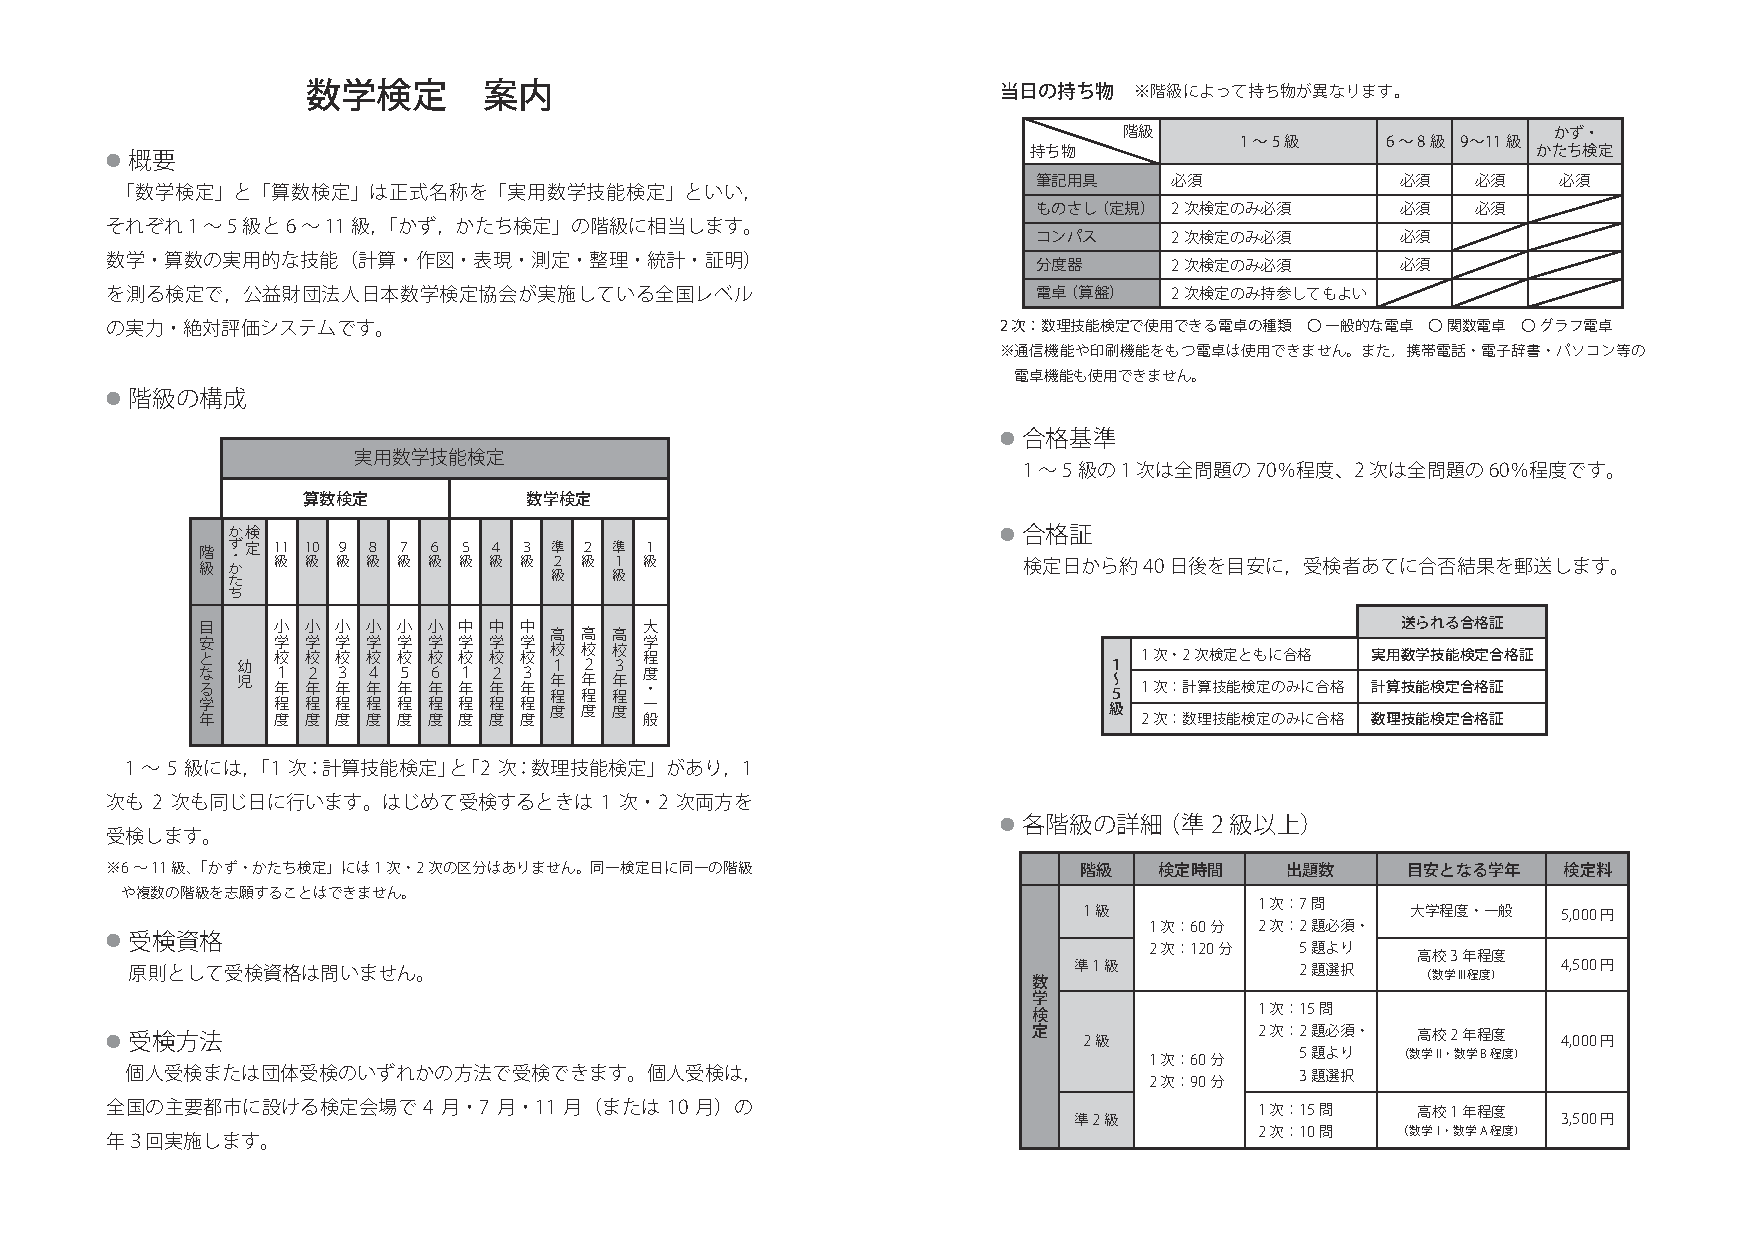
\includegraphics[trim=0 0 148.5mm 0,clip]{./KenteiAnnai/KenteiAnnai.pdf}
\vss}
\end{center}%%\thispagestyle{empty}%
\newpage
\begin{center}
\centering%%\thispagestyle{empty}%
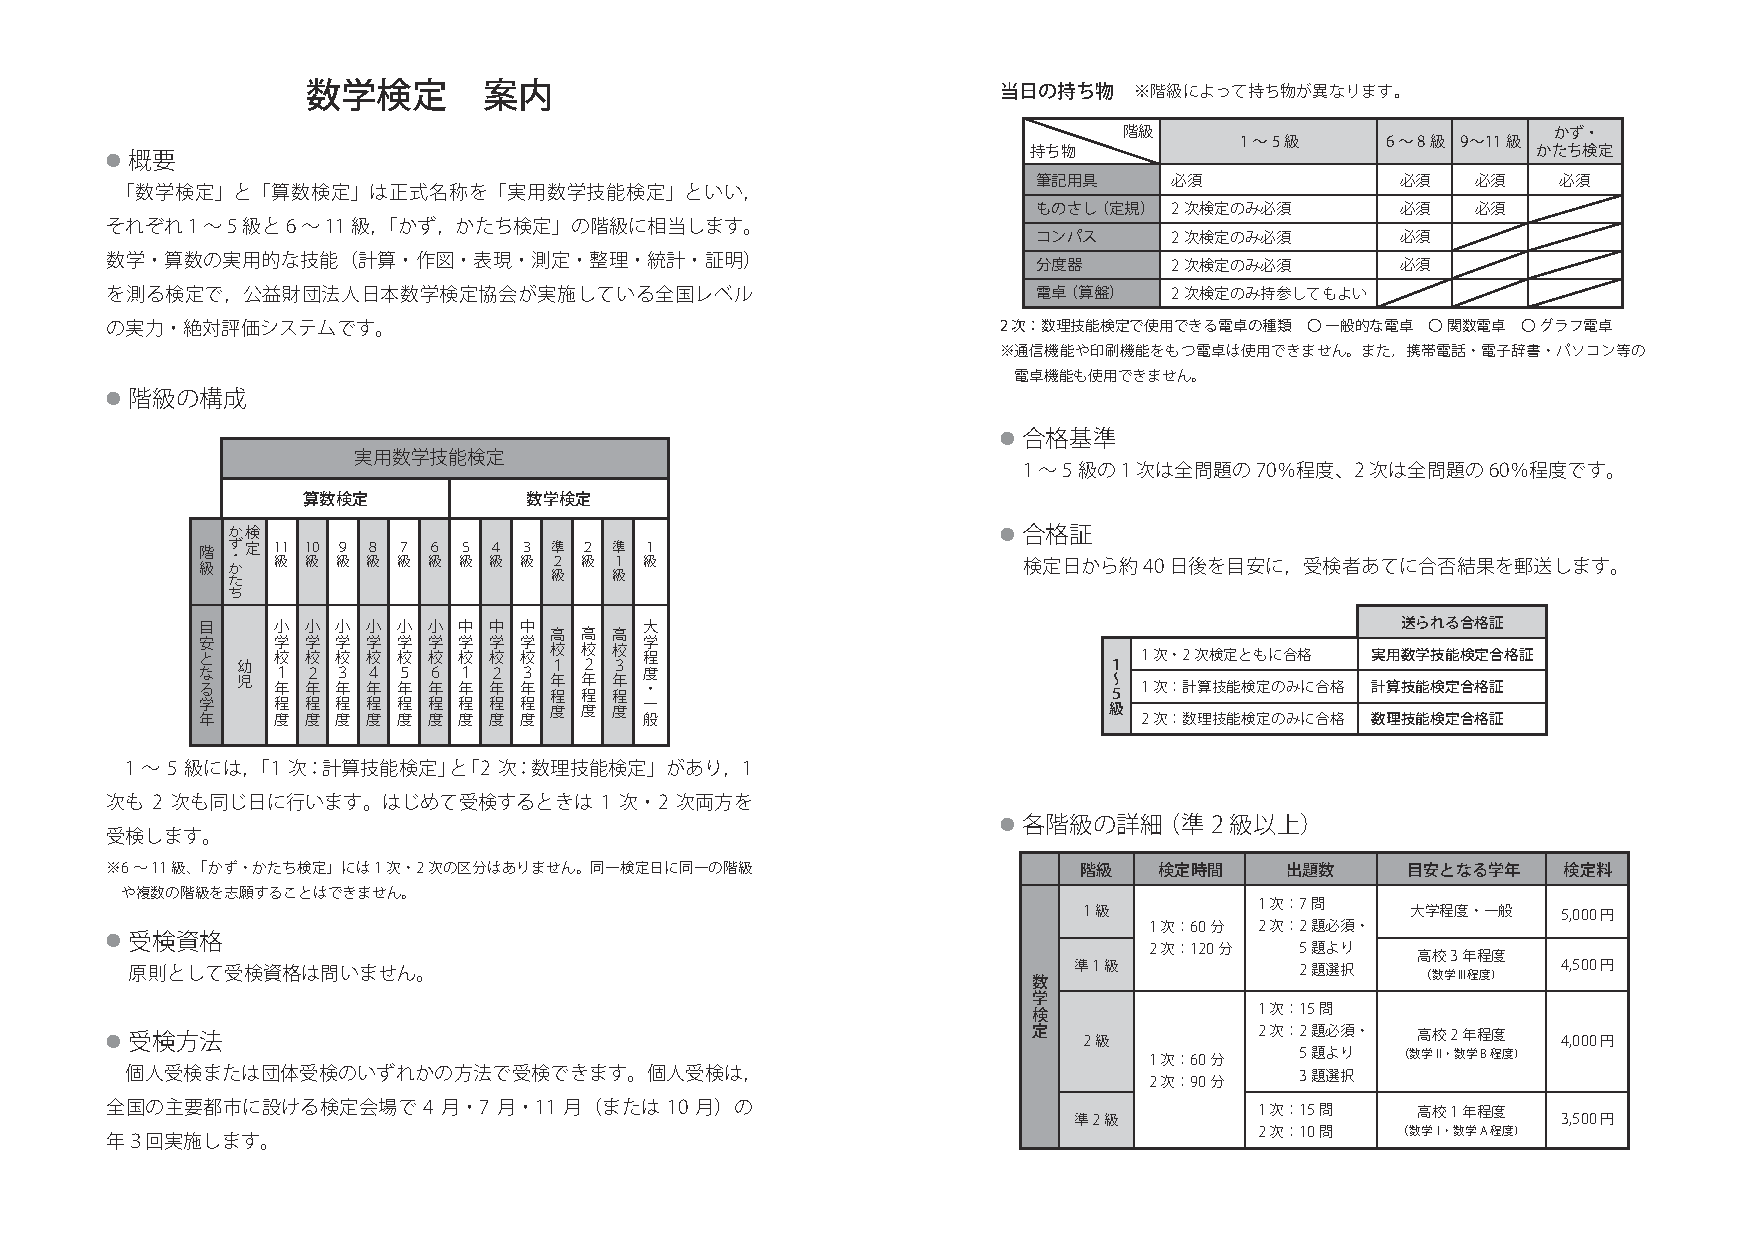
\includegraphics[trim=148.5mm 0 0 0,clip]{./KenteiAnnai/KenteiAnnai.pdf}
\end{center}
\newpage
\tableofcontents
\mainmatter
\setcounter{chapter}{-1}
\chapter{計算テクニック}
\newcommand\Binom[2]{\bigg(\begin{array}{@{\,}c@{\,}}#1\\[-.5mm]#2\end{array}\bigg)}

\section{高次方程式}
\step{基本を確認しておこう}


高次方程式 $P(x)=0$ を解くには,主に次の3つの手法を用いる.

\begin{enumerate}
\item[a.] 因数分解の公式を利用する
\item[b.] \<($x$の2次式)\<$=X$ の形に置き換えて次数を下げる
\item[c.] 因数定理を用いて,$P(x)$ を1次または2次の積に直す
\end{enumerate}
\begin{titlebox}{因数定理}
$\begin{array}{ll}
\text{整式$P(x)$が$x-a$を因数にもつ}&\Longleftrightarrow P(a)=0\\
\text{整式$P(x)$が1次式$ax-b$を因数にもつ}&\Longleftrightarrow P\left (\frac{b}{a}\right )=0
\end{array}$\\
\end{titlebox}
\begin{例}
$P(x)=2x^{3}-7x^{2}+6x+5=0$ を解いてみよう.
\end{例}
\begin{解}
1つの有理数解 $x=\frac{b}{a}$($a$ と $b$ は互いに素で,$a$ は自然数,$b$ は整数)を見い出すには,$x=\pm\frac{P(x)\text{の定数項の正の約数}}{P(x)\text{の最高次の係数の正の約数}}$ の中から探せばよい.

\noindent
$x=\pm\frac{\text{5の正の約数}}{\text{2の正の約数}} =\pm\frac{1,5}{1,2}$ より $x=\pm 1, \pm 5, \pm\frac{1}{2}, \pm\frac{5}{2}$ を考えて
\[
P\left (-\frac{1}{2}\right )=2\cdot\left (-\frac{1}{8}\right )-7\cdot\frac{1}{4}+6\cdot\left (-\frac{1}{2}\right )+5=-2-3+5=0
\]%%\newpage
\begin{Mw}{40mm}{%
%\arraycolsep.5zw$
%\begin{array}{rrrrr}
%\multicolumn{1}{r|}{-\dfrac{1}{2\rule[-1mm]{0pt}{0pt}}}&2&-7&6&5\\
%\cline{1-1}
%&&-1&4&-5\\
%\hline
%&2&-8&10&\multicolumn{1}{|r}{0}\\
%\cline{5-5}
%\end{array}$
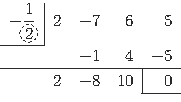
\includegraphics{./fig/fig00-step01}
}
これにより
\begin{align*}
P(x)&=\left (x+\frac{1}{2}\right )(2x^{2}-8x+10)\\
&=(2x+1)(x^{2}-4x+5)=0
\end{align*}
よって,$x=-\frac{1}{2},\ 2\pm i$
\end{Mw}

{\footnotesize
右上の計算は,$x$の整式を1次式$x-\alpha$で割ったときの商と余りを求める方法で,「組立除法」と呼ばれる.
たとえば,「$(x^3-3x+2)\div(x-2)$の商と余りは?」ならば,
割る数$x-2$が0となる$x={\fboxsep.1zw\colorbox[gray]{.9}{$2$}}$と整数の係数\,{\fboxsep.1zw\colorbox[gray]{.9}{$1 \quad 0 \quad -3 \quad 2$}}\,を
\[
\raisebox{0pt}[0pt][0pt]{\def\arraystretch{0.85}\begin{array}[t]{@{\ }c@{\ }|}%
\rule{0pt}{1.5ex}2\\[0pt]\hline
\end{array}} \quad 1 \quad 0 \quad -3 \quad 2
\]
\begin{Mw}(0pt,9mm){48mm}{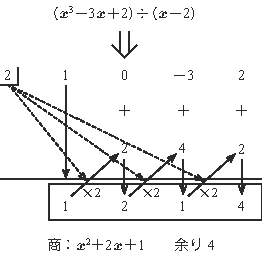
\includegraphics{./fig/sec00_betsu01.pdf}}
\noindent
と書き並べるところから始める.
左から順に

\vspace{.5\baselineskip}
1. 1を下ろす$\Rightarrow$\ajKaku{1}

2. $\ajKaku{1}\times 2\Rightarrow2$

3. $0+2\Rightarrow$\ajKaku{2}

4. $\ajKaku{2}\times 2\Rightarrow4$

5. $(-3)+4\Rightarrow$\ajKaku{1}

6. $\ajKaku{1}\times 2\Rightarrow$2

7. $2+2\Rightarrow$\ajKaku{4}(余り)

\vspace{.5\baselineskip}
\noindent
のように計算すると,商と余りを簡単に求めることができる.
高次方程式$P(x)=0$を解く際,$P(\alpha)=0$となる$\alpha$を見出して,組立除法を用いると,$P(x)=(x-\alpha)P_1(x)=0$と変形することができ,次数を下げられる.
\par
\end{Mw}
}

\end{解}
\step{基本問題を解いてみよう}
\begin{例題}
次の高次方程式を解け.
\begin{longtable}[l]{@{}l@{\hskip4zw}l}
(1)\hspace{1zw}$2x^{3}-x^{2}-13x-6=0$\hspace{4zw}&
(2)\hspace{1zw}$3x^{3}-4x^{2}+2x+4=0$ \\
 (3)\hspace{1zw}$x^{4}-4x+3=0$&
\end{longtable}
\end{例題}

\begin{解答}
方程式の左辺を $P(x)$ とおく.\\[3mm]
\begin{fleqn}[4zw]
(1) $\Mframe{P(-2)}=-16-4+26-6\,\Mframe{=0}$\Footnote{有理数解の候補は$x=\pm\frac{-6\text{の正の約数}}{\text{2の正の約数}}=\pm\frac{1,2,3,6}{1,2}$}\\
$P(x)$を$x+2$で割ると,商は $2x^{2}-5x-3$
\[
P(x)=(x+2)(2x^{2}-5x-3)=(x+2)(2x+1)(x-3)=0
\]
よって,$x=-2, -\frac{1}{2},3$\kotae
\end{fleqn}

\begin{fleqn}[4zw]
(2) $P\left (-\frac{2}{3}\right )=3\cdot\left (-\frac{8}{27}\right )-4\cdot\frac{4}{9}+2\cdot\left (-\frac{2}{3}\right )+4=0$\\
\hspace{1zw}$P(x)$を$3x+2$で割ると,商は $x^{2}-2x+2$
\begin{alignat}{1}
P(x)=(3x+2)(x^{2}-2x+2)=0\notag
\end{alignat}
よって,$x=-\frac{2}{3}, 1\pm i$\kotae
\end{fleqn}
\begin{fleqn}[4zw]
(3) $P(1)=1-4+3=0$\\
$P(x)$を$x-1$で割ると,商は $Q(x)=x^{3}+x^{2}+x-3$
\begin{alignat}{1}
P(x)=(x-1)(x^{3}+x^{2}+x-3)\notag
\end{alignat}
さらに $Q(1)=1+1+1-3=0$ だから
\begin{alignat}{1}
Q(x)=(x-1)(x^{2}+2x+3)\notag
\end{alignat}
したがって
\begin{alignat}{1}
P(x)=(x-1)^{2}(x^{2}+2x+3)\notag
\end{alignat}
よって,$x=1$ (2重解),\ $-1\pm\sqrt{2}i$\kotae
\end{fleqn}
\end{解答}

\vspace{.5\baselineskip}\noindent
%%\fbox{※コラム入る}
\begin{center}
{\footnotesize
\begin{tabular}{@{}c@{}}\tabcolsep.75\tabcolsep
(1)\ \begin{tabular}[t]{>{$}r<{$}>{$}r<{$}>{$}r<{$}>{$}r<{$}>{$}r<{$}}
\multicolumn{1}{r|}{$-2$} & 2 & -1 & -13 & -6\\
\cline{1-1}
   &   & -4 &  10&  6\\
   \hline
   & 2 & -5 &\multicolumn{1}{r|}{$-\phantom{1}3$}&  0\\
   \cline{5-5}
\multicolumn{5}{l}{商 $2x^2-5x-3$}
\end{tabular}\quad\hskip2mm
(2)\ \begin{tabular}[t]{>{$}r<{$}>{$}r<{$}>{$}r<{$}>{$}r<{$}>{$}r<{$}}
\multicolumn{1}{r|}{$-\dfrac{2}{3}$} & 3 & -4 & 2 & 4\\[2mm]
\cline{1-1}
\multicolumn{5}{r}{}\\[-6.5mm]
   &   & -2 & 4&  -4\\
   \hline
   & 3 & -6 &\multicolumn{1}{r|}{$6$}&  0\\
   \cline{5-5}
\multicolumn{5}{l}{商 $x^2-2x+2$}
\end{tabular}\quad\hskip2mm
(3)\ \begin{tabular}[t]{>{$}r<{$}>{$}r<{$}>{$}r<{$}>{$}r<{$}>{$}r<{$}>{$}r<{$}}
\multicolumn{1}{r|}{$1$} & 1 & 0 & 0 & -4 & $3$\\
\cline{1-1}
   &   & 1 & 1 &  1 & -3 \\
\hline
\multicolumn{1}{r|}{$1$} & 1 & 1 & 1 & \multicolumn{1}{r|}{$-3$} & 0\\
   \cline{1-1}\cline{6-6}
& & 1 & 2 & 3 & \\
\cline{1-5}
&  1 & 2 &\multicolumn{1}{r|}{$3$} &0 &\\
\cline{5-5}
\multicolumn{6}{@{}l}{\hbox to2zw{\rule{0pt}{1.2zh}商 $x^2+2x+3$}}
\end{tabular}
\end{tabular}
}
\end{center}

\vspace{-4mm}
%%\clearpage
\section{極形式}
\step{基本を確認しておこう}

%\begin{Mw}<6>[+3]{35mm}{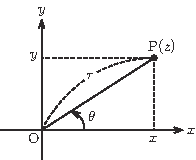
\includegraphics{./fig/sec00_2_1.pdf}}
複素平面上で,$0$ でない複素数 $z=x+yi$
を表す点を $\mathrm{P}$ とし,$\overrightarrow{\OP}$ と実軸の正の向きとのなす角
を $\theta$, $\overline{\OP}$ $=|z|=r$ とすると
\[
 x=r\cos\theta,\ y=r\sin\theta
\]

\begin{fleqn}
\[
\text{すなわち,}\ z=r(\cos\theta+i\sin\theta)\hspace{1zw}(r>0)\tag*{……①}
\]
\end{fleqn}\pagebreak[3]


\begin{Mw}[+1]{35mm}{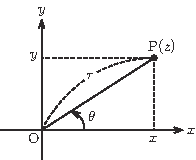
\includegraphics{./fig/sec00_2_1.pdf}}
\hspace*{-1zw}と表される.①のような表し方を,複素数 $z$ の\textbf{極形式}という.$r$ を $z$ の絶対値,$\theta$ を $z$ の\textbf{偏角}といい,$\arg z$ で表す.$\arg$はargument の略である.
\[
r=|z|,\hspace{1zw}\theta=\arg z
\]
\textbf{[1]}\hspace{1zw}\textbf{偏角}\hspace{1zw}複素数 $z$ の偏角は,$\overrightarrow{\mathrm{OP}}$ が実軸の正の向きとなすどのような角でもよく,一般角で考えることもある.$\theta$ が $z$ の1つの偏角なら
\[
\theta+2 n\pi \hspace{1zw} (n=0, \pm 1, \pm 2, \ldots)
\]
はすべて$z$の偏角であり,逆に,$z$のどの偏角もこの形で表せる.
\end{Mw}

また,$z=0$ のとき偏角は定まらないので,$\arg 0$ は考えないことにする.
さらに,$z=r(\cos\theta+i\sin\theta)$ のとき
\[
\overline{z}=r(\cos\theta-i\sin\theta)=r\{\cos(-\theta)+i\sin(-\theta)\}
\]
だから\hspace{3zw} $|\overline{z}|=|z|$\hspace{1zw}かつ\hspace{1zw}$\arg\overline{z}=-\arg z$

\begin{fleqn}
\begin{alignat*}{1}
\text{2つの複素数} z_{1}=r_{1}(\cos\theta_{1}+i\sin\theta_{1}) , z_{2}=r_{2}(\cos\theta_{2}+i\sin\theta_{2})\tag*{……②}
\end{alignat*}
\end{fleqn}


\noindent
のとき\hspace{2zw}$z_{1}=z_{2}\hspace{1zw}\Longleftrightarrow\hspace{1zw} r_{2}=r_{1}$ かつ $\theta_{2}=\theta_{1}+2n\pi\hspace{1zw}(n\in \mathbb{Z})$

\noindent
\textbf{[2]}\hspace{1zw}\textbf{極形式と乗法・除法}\hspace{1zw}②をみたす2つの複素数 $z_{1}$, $z_{2}$について
\begin{fleqn}[4zw]
\begin{alignat}{1}
z_{1}z_{2}&=r_{1}(\cos\theta_{1}+i\sin\theta_{1})\cdot r_{2}(\cos\theta_{2}+i\sin\theta_{2})\notag\\
&=r_{1}r_{2}\{(\cos\theta_{1}\cos\theta_{2}-\sin\theta_{1}\sin\theta_{2})\notag\\
&\phantom{=\;} +i(\sin\theta_{1}\cos\theta_{2}+\cos\theta_{1}\sin\theta_{2})\}\notag
\end{alignat}
\end{fleqn}
\hspace{0zw}$\text{より}\hspace{2zw}\quad z_{1}z_{2}=r_{1}r_{2}\{\cos(\theta_{1}+\theta_{2})+i\sin(\theta_{1}+\theta_{2})\}$

\noindent
\begin{fleqn}
\begin{alignat*}{3}
\text{すなわち}&\hspace{3zw}&&|z_{1}z_{2}|= |z_{1}||z_{2}|,\ \arg(z_{1}z_{2})=\arg z_{1}+\arg z_{2}\tag*{……③}
\end{alignat*}
\end{fleqn}
同様にして\hspace{2zw}$\left |\frac{z_{1}}{z_{2}}\right |=\frac{|z_{1}|}{|z_{2}|},\hspace{1zw}\arg\left (\frac{z_{1}}{z_{2}}\right )=\arg z_{1}-\arg z_{2}$\hspace{2zw}が成り立つ.

\pagebreak
\step{基本問題を解いてみよう}
\begin{例題}
次の複素数を極形式で表せ.\par
\begin{longtable}[l]{@{}l@{\hskip4zw}l}
(1)\quad$z=-\frac{5}{2}i\ $&$(2)\quad z=\frac{-5+i}{2-3i}$
\end{longtable}
\end{例題}

\begin{解答}
%\begin{Mw}{26mm}{\Fig{26mm}{24mm}}
\begin{Mw}{26mm}{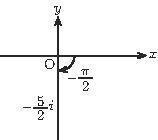
\includegraphics{./fig/sec00_2_2.pdf}}
(1)\hskip1zw$z=-\frac{5}{2}i$\\
$=\frac{5}{2}\left \{\cos\left (-\frac{\pi}{2}\right )+i\sin\left (-\frac{\pi}{2}\right )\right \}$\kotae
\begin{fleqn}[0zw]
\begin{alignat}{3}
(2)\hskip1zwz&=&&\frac{-5+i}{2-3i}=\frac{(-5+i)(2+3i)}{(2-3i)(2+3i)}\notag\\[3mm]
&=&&\frac{-13-13i}{13}=-1-i\notag
\end{alignat}
\end{fleqn}
\end{Mw}
よって,$z=\sqrt{2}\left (\cos\frac{5}{4}\pi+i\sin\frac{5}{4}\pi\right )$\kotae
\end{解答}

\section{$\boldsymbol{n}$乗根}
\step{基本を確認しておこう}
\begin{fleqn}
\begin{equation}
\hspace{1zw}\text{$n$を正の整数とする.複素数}\ \alpha\,(\neq 0) に対して\hspace{2zw}z^{n}=\alpha
\end{equation}
\end{fleqn}
をみたす複素数 $z$ を $\alpha$ の $\boldsymbol{n}$\textbf{乗根}という.

%\begin{Mw}{28mm}{\Fig{28mm}{30mm}}
\begin{Mw}{28mm}{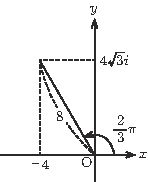
\includegraphics{./fig/sec00_3_1.pdf}}
$z^{3}=-4+4\sqrt{3}i$ をみたす複素数 $z$ を求めてみよう.
\begin{fleqn}[4zw]
\begin{alignat}{2}
&|-4+4\sqrt{3}i|=\sqrt{(-4)^{2}+(4\sqrt{3})^{2}}=8\notag\\
&\arg(-4+4\sqrt{3}i)=\frac{2}{3}\pi+2n\pi\notag
\end{alignat}
\end{fleqn}
だから\hspace{1zw}$-4+4\sqrt{3}i=8\left (\cos\frac{2}{3}\pi+i\sin\frac{2}{3}\pi\right )$

$z=r(\cos\theta+i\sin\theta)\, (r>0,\ 0\leqq\theta<2\pi)$ とおくと,ド・モアブルの定理から,
方程式は
\end{Mw}
\[
r^{3} (\cos 3\theta+i$ sin3 $\theta)=8\left(\cos\dfrac{2}{3}\pi+i\sin\dfrac{2}{3}\pi\right)
\]%
\settowidth{\dimen0}{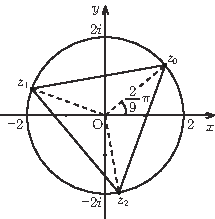
\includegraphics{./fig/0.pdf}}%
\begin{Mw}{\dimen0}{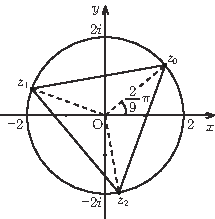
\includegraphics{./fig/0.pdf}}
両辺の絶対値および偏角を比べて
\[
\hspace{1.5zw}r^{3}=8,\hspace{1zw}3\theta=\frac{2}{3}\pi+2n\pi\par
\]
\hspace{2zw}$\therefore \hspace{1zw} r=2,\hspace{1zw}\theta=\frac{2}{9}\pi+\frac{2n}{3}\pi$\\[3mm]
$ 0\leqq\theta<2\pi$ では \hspace{1.5zw}$\theta=\frac{2}{9}\pi,\ \frac{2}{9}\pi+\frac{2}{3}\pi,\ \frac{2}{9}\pi+\frac{4}{3}\pi$
\begin{fleqn}
\begin{alignat}{3}
よって\hspace{1zw}& z_{0}=2\left (\cos\frac{2}{9}\pi+i\sin\frac{2}{9}\pi\right ),&\notag\\[3mm]
&z_{1}=2\left (\cos\frac{8}{9}\pi+i\sin\frac{8}{9}\pi\right ),&\quad z_{2}=2\left (\cos\frac{14}{9}\pi+i\sin\frac{14}{9}\pi\right )\notag
\end{alignat}
\end{fleqn}

これらの3乗根は,複素平面上で点O(0) を中心とし,半径 $\sqrt[3]{8}=2$ の円周を3等分した点 (半径2の円に内接する正3角形の3頂点) になる.同様に,
\end{Mw}

$\alpha=r_{0}(\cos\theta_{0}+i\sin\theta_{0})$ のとき,①をみたす $n$ 乗根$z$は $n$ 個あり
\begin{align*}
z_k&=\sqrt[n]{r_{0}}\left \{\cos\left (\frac{\theta_{0}}{n}+\frac{2k\pi}{n}\right )+i\sin\left (\frac{\theta_{0}}{n}+\frac{2k\pi}{n}\right )\right \}\\
&\phantom{=\;}\;(k=0,1,\ldots,n-1)
\end{align*}
となる.複素平面上で,点 $z_{k}\, (k=0,1,\ldots,n-1)$ は点O(0) を中心とし,半径$\sqrt[n]{r_{0}}$ の円周を $n$ 等分した点になる.

\step{基本問題を解いてみよう}
\begin{例題}
次の複素数を求めよ.\vs{-1.5mm}\par
\begin{longtable}[l]{@{}l@{\hskip4zw}l}
(1)\hspace{.5zw} $i$ の平方根&(2) \hspace{.5zw}$-2+2\sqrt{3}i$ の4乗根
\end{longtable}\vs{-1.5mm}
\end{例題}

\begin{解答}
\vspace{-\baselineskip}\vspace{-\abovedisplayskip}
\begin{fleqn}[4zw]
\vspace{\baselineskip}\vspace{\abovedisplayskip}
(1)\hskip1zw$i=\cos\frac{\pi}{2}+i\sin\frac{\pi}{2}$\par
\noindent
$z^{2}=i$ をみたす$z$は2個あり

\begin{alignat}{2}
z_k & =\cos\left(\frac{\pi}{4}+k\pi\right)+
i\sin\left(\frac{\pi}{4}+k\pi\right)\quad(k=0,1)\notag\\
z_{0}&=\cos\frac{\pi}{4}+i\sin\frac{\pi}{4}=\frac{1}{\sqrt{2}}(1+i)\notag\\[3mm]
z_{1}&=\cos\frac{5}{4}\pi+i\sin\frac{5}{4}\pi=-\frac{1}{\sqrt{2}}(1+i)\tag*{\kotae}
\end{alignat}
\end{fleqn}
\begin{fleqn}[4zw]
(2)\hspace{1zw} $-2+2\sqrt{3}i=4\left (\cos\frac{2}{3}\pi+i\sin\frac{2}{3}\pi\right )$\par\noindent
$z^{4}=-2+2\sqrt{3}i$ をみたす$z$ は4個あり
\end{fleqn}
\begin{fleqn}[1zw]
\begin{alignat*}{2}
z_{0}&=\sqrt[4]{4}\left (\cos\frac{1}{6}\pi+i\sin\frac{1}{6}\pi\right )=\sqrt{2}\left( \frac{\sqrt{3}}{2}+\frac{1}{2}i\right) = \frac{\sqrt{6}}{2}+\frac{\sqrt{2}}{2}i\\[3mm]
z_{1}&=\sqrt[4]{4}\left (\cos\frac{2}{3}\pi+i\sin\frac{2}{3}\pi\right )
=\sqrt{2}\left (-\frac{1}{2}+\frac{\sqrt{3}}{2}i\right )=-\frac{\sqrt{2}}{2}+\frac{\sqrt{6}}{2}i\\[3mm]
z_{2}&=\sqrt[4]{4}\left (\cos\frac{7}{6}\pi+i\sin\frac{7}{6}\pi\right )=\sqrt{2}\left( -\frac{\sqrt{3}}{2}-\frac{1}{2}i \right) =-\frac{\sqrt{6}}{2}-\frac{\sqrt{2}}{2}i \\[3mm]
z_{3}&=\sqrt[4]{4}\left (\cos\frac{5}{3}\pi+i\sin\frac{5}{3}\pi\right )
=\sqrt{2}\left (\frac{1}{2}-\frac{\sqrt{3}}{2}i\right )=\frac{\sqrt{2}}{2}-\frac{\sqrt{6}}{2}i\hspace{.5zw}{\kotae}
\end{alignat*}
\end{fleqn}
\end{解答}

\section{3次方程式の一般的解法}
\step{基本を確認しておこう}
ここでは,3次方程式 $a_{0}x^{3}+a_{1}x^{2}+a_{2}x+a_{3}=0\ (a_{0}\neq 0)$
\hfill{……①} \\
について学ぶ.係数は(最初は)整数とする.
\setcounter{equation}{2}

①が有理数の解をもたないときを考える.①の両辺を $a_{0}$ で割って
\[
x^{3}+ax^{2}+bx+c=0\ \left (a=\frac{a_{1}}{a_{0}},\hspace{1zw}b=\frac{a_{2}}{a_{0}},\hspace{1zw}c=\frac{a_{3}}{a_{0}}\right )
\]
の形になるが,$x^{2}$ の項を消去するために,$x=y-\frac{a}{3}$ とおくと,
\begin{align*}
\left (y-\frac{a}{3}\right )^{3}&+a\left (y-\frac{a}{3}\right )^{2}+b\left (y-\frac{a}{3}\right )+c=0\notag\\
\intertext{これを整理し,
$p=-\frac{a^{2}}{3}+b,\ q=\frac{2}{27}a^{3}-\frac{ab}{3}+c$とおくと}
 y^{3}&+py+q=0\tag*{……②}
\end{align*}
となる.さらに,$y=u+v$ とおくと\hspace{2zw}$(u+v)^{3}+p(u+v)+q=0$
\[
u^{3}+v^{3}+q+(u+v)(3uv+p)=0
\]
{\mathindent0pt
\begin{empheq}[left=となるので\hspace{1zw}\empheqlbrace]{alignat=1}
&u^{3}+v^{3}+q=0 \\
&3uv+p=0
\end{empheq}}%\vspace{.25\baselineskip}

\noindent
を満たす $u$ と $v$ の値を求めることができれば,$y=u+v$ から $y$, さらに
$x=y-\frac{a}{3}$ から①の解 $x$ が得られる.実際に $u, v$ は③,④からそれぞれ

\[
u^{3}+v^{3}=-q,\qquad u^{3}v^{3}=(uv)^{3}=\left (-\frac{p}{3}\right )^{3}=-\frac{p^{3}}{27}\]
となるので,$u^{3}$ と $v^{3}$ は $t$ の2次方程式 $(t-u^{3})(t-v^{3})=0$ の解,すなわち
\begin{fleqn}[4zw]
\begin{alignat}{1}
t^{2}+qt-\frac{p^{3}}{27}=0
\end{alignat}
\end{fleqn}
の解として得られる.⑤を①の\textbf{分解方程式}と呼ぶ.さて,⑤を解くと
\begin{align*}
t=\frac{1}{2}\left (-q\pm\sqrt{q^{2}+\frac{4}{27}p^{3}}\right )=-\frac{q}{2}\pm\sqrt{\frac{q^{2}}{4}+\frac{p^{3}}{27}}
\end{align*}
となるので,$\frac{q^{2}}{4}+\frac{p^{3}}{27}=r$ とすると,$u^{3}=-\frac{q}{2}+\sqrt{r},\hspace{1zw}v^{3}=-\frac{q}{2}-\sqrt{r}$\par
\noindent
ここで,$u^{3}=A^{3}$ ($A$ は定数) を解くと
\begin{align*}
(u-A)(u^{2}+Au+A^{2})=0\hspace{1zw}から,\ u=A, \frac{-1\pm\sqrt{3}i}{2}A
\end{align*}

$\frac{-1+\sqrt{3}i}{2}=\ruby{$\omega$}{オメガ}$とおくと,\ $\omega^{2}=\left (\frac{-1+\sqrt{3}i}{2}\right )^{2}=\frac{-1-\sqrt{3}i}{2}$ となるので $u^{3}=A^{3}$ の3解は $u=A,\ \omega A,\ \omega^{2}A$ となる.


したがって,$1+\omega+\omega^{2}=0$ に注意すると ③, ④を満たす $u, v$ の値は
\begin{alignat*}{2}
u&=\sqrt[3]{-\frac{q}{2}+\sqrt{r}}, & v&=\sqrt[3]{-\frac{q}{2}-\sqrt{r}}\\[3mm]
u&=\omega\sqrt[3]{-\frac{q}{2}+\sqrt{r}},& v&=\omega^{2}\sqrt[3]{-\frac{q}{2}-\sqrt{r}}\\[3mm]
u&=\omega^{2}\sqrt[3]{-\frac{q}{2}+\sqrt{r}},\qquad& v&=\omega\sqrt[3]{-\frac{q}{2}-\sqrt{r}}
\end{alignat*}
の3組となる.これを $y=u+v$ に代入すると,下に示した3組の $y$, すなわち②の3解
が得られ,①の3解が求められる.
\[\left\{
	\begin{array}{lll}
y_{1}&=\sqrt[3]{-\dfrac{q}{2}+\sqrt{r}}\ & +\;\sqrt[3]{-\dfrac{q}{2}-\sqrt{r}}\\[3mm]
y_{2}&=\omega\sqrt[3]{-\dfrac{q}{2}+\sqrt{r}}\ &+\;\omega^{2}\sqrt[3]{-\dfrac{q}{2}-\sqrt{r}}\\[3mm]
y_{3}&=\omega^{2}\sqrt[3]{-\dfrac{q}{2}+\sqrt{r}}\ &+\;\omega\sqrt[3]{-\dfrac{q}{2}-\sqrt{r}}
\end{array}\right.
\]
\pagebreak

\step{基本問題を解いてみよう}
\begin{例題}
次の3次方程式を解け.\par
\begin{longtable}[l]{l@{\hskip4zw}l}
(1)\hspace{1zw}$x^{3}+6x+2=0$ & (2)\hspace{1zw}$x^{3}+3x^{2}-3=0$
\end{longtable}
\end{例題}

\begin{解答}
%\vspace{-\baselineskip}\vspace{-\abovedisplayskip}
(1)\hspace{1zw}$\Mframe{x=u+v\text{とおく}}\Footnote{$x^2$の項はないので,このまま$x=u+v$とおける.}$と\vspace{-\abovedisplayskip}\par
\begin{fleqn}[4zw]
\begin{align*}
&(u+v)^{3}+6(u+v)+2=0\\
&u^{3}+v^{3}+2+(u+v)(3uv+6)=0\\
&\left\{\begin{array}{@{}l}
u^{3}+v^{3}+2=0\\
3uv+6=0
\end{array}\right.
\Longleftrightarrow
\left\{\begin{array}{@{}l}
u^{3}+v^{3}=-2\\
uv=-2
\end{array}\right.
\Longrightarrow
\left\{\begin{array}{@{}l}
u^{3}+v^{3}=-2\\
u^3v^3=(-2)^3=-8
\end{array}\right.
\end{align*}
を満たす $u^{3}$ と $v^{3}$ は $t^{2}+2t-8=0$ の2解である.
\[
(t-2)(t+4)=0$\hspace{1zw}から,$t=2, -4
\]
したがって,1組の $u, v$ は
\[
u=\sqrt[3]{2},\ v=\sqrt[3]{-4}=-\sqrt[3]{4}
\]
よって,求める解 $x=x_{i}\,(i=1,2,3)$ は
\begin{fleqn}[1zw]
\begin{align*}
&\left\{\begin{array}{l}
x_{1}=u+v=\sqrt[3]{2}-\sqrt[3]{4}\\
x_{2}=\omega u+\omega^{2}v=\sqrt[3]{2}\omega-\sqrt[3]{4}\omega^{2}\\
x_{3}=\omega^{2}u+\omega v=\sqrt[3]{2}\omega^{2}-\sqrt[3]{4}\omega
\end{array}\right. \left (\text{ただし,}\omega=\frac{-1+\sqrt{3}i}{2}\right )
\tag*{\Kotae}
\end{align*}
\end{fleqn}
(2)\hspace{1zw}$\Mframe{x=y-1\text{とおく}}\Footnote{$x^2$の項をなくすために,$x=y-1$とおく.}$と,$(y-1)^{3}+3(y-1)^{2}-3=0$
から,$y^{3}-3y-1=0$\par
\noindent
$y=u+v$ とおくと,$(u+v)^{3}-3(u+v)-1=0$
\[
u^{3}+v^{3}-1+(u+v)(3uv-3)=0
\]
\[
\left\{\begin{array}{@{}l}
u^{3}+v^{3}-1=0\\
3uv-3=0
\end{array}\right.
\Longleftrightarrow
\left\{\begin{array}{@{}r}
u^{3}+v^{3}=1\\
uv=1
\end{array}\right.
\Longrightarrow
\left\{\begin{array}{@{}r}
u^{3}+v^{3}=1\\
u^3v^3=1
\end{array}\right.
\]
を満たす $u^{3}$ と $v^{3}$ は,$t^{2}-t+1=0$ を解いて
\begin{alignat}{2}
t&=\frac{1\pm\sqrt{3}i}{2}=\cos\left (\pm\frac{\pi}{3}\right )+i\sin\left (\pm\frac{\pi}{3}\right )\hspace{2zw}\text{(複号同順)}\notag\\
\intertext{よって}
u^{3}&=\cos\frac{\pi}{3}+i\sin\frac{\pi}{3},\qquad
v^{3}=\cos\left (-\frac{\pi}{3}\right )+i\sin\left (-\frac{\pi}{3}\right )\notag
\end{alignat}
これを満たす1組の $u, v$ は,ド・モアブルの定理から
\[
u=\cos\frac{\pi}{9}+i\sin\frac{\pi}{9},\ v=\cos\left (-\frac{\pi}{9}\right )+i\sin\left (-\frac{\pi}{9}\right )
\]
より,求める$y$の値は
\begin{align*}
y_{1}&=u+v=2\cos\frac{\pi}{9}\\
y_{2}&=\left (\cos\frac{2}{3}\pi+i\sin\frac{2}{3}\pi\right )\left (\cos\frac{\pi}{9}+i\sin\frac{\pi}{9}\right )\\
&\phantom{=\;} +\left\{\cos\left (-\frac{2}{3}\pi\right )+i\sin\left (-\frac{2}{3}\pi\right)\right\}\left\{\cos\left (-\frac{\pi}{9}\right )+i\sin\left (-\frac{\pi}{9}\right )\right\}\\
&=\cos\frac{7}{9}\pi+i\sin\frac{7}{9}\pi
+\cos\left (-\frac{7}{9}\pi\right )+i\sin\left (-\frac{7}{9}\pi\right )\\
&=2\cos\frac{7}{9}\pi
\end{align*}
同様に,$ y_{3}=\omega^{2}u+\omega v=2\cos\frac{13}{9}\pi$
\par\noindent
よって,
\[
x_{1} = 2\cos\frac{\pi}{9} -1,\quad
x_{2} = 2\cos\frac{7}{9}\pi -1,\quad
x_{3} = 2\cos\frac{13}{9}\pi -1
\kotae\]
\end{fleqn}
\end{解答}

\section{三角関数}
\step{基本を確認しておこう}
2つの角の和または差の三角関数の値を求めるには,次の加法定理を用いる.
\begin{titlebox}{加法定理}
\begin{fleqn}[4zw]
\begin{align*}
\sin(\alpha + \beta)=&\sin\alpha\cos\beta + \cos\alpha\sin\beta\tag*{……①}\\
\sin(\alpha - \beta)=&\sin\alpha\cos\beta - \cos\alpha\sin\beta\tag*{……②}\\
\cos(\alpha + \beta)=&\cos\alpha\cos\beta - \sin\alpha\sin\beta\tag*{……③}\\
\cos(\alpha - \beta)=&\cos\alpha\cos\beta + \sin\alpha\sin\beta\tag*{……④}\\
\tan(\alpha + \beta)=&\dfrac{\tan\alpha + \tan\beta}{1 - \tan\alpha\tan\beta}\tag*{……⑤}\\[3mm]
\tan(\alpha - \beta)=&\dfrac{\tan\alpha - \tan\beta}{1 + \tan\alpha\tan\beta}\tag*{……⑥}
\end{align*}
\end{fleqn}
\end{titlebox}

①,③,⑤で $\alpha=\beta=\theta$ とおくと,次の2倍角の公式が得られる.


\begin{titlebox}{2倍角の公式}
\begin{fleqn}[4zw]
\[
\begin{array}{llr}
\sin 2\theta&= 2\sin\theta\cos\theta&\\[1mm]
\cos 2\theta&= \cos^2\theta - \sin^2\theta = 2\cos^2\theta - 1 
= 1-2\sin^2\theta\\
\tan2\theta&= \dfrac{2\tan\theta}{1-\tan^2\theta}&
\end{array}\tag*{……⑦}
\]
\end{fleqn}
\end{titlebox}

特に,$\tan\theta=m$ とおくとき,次は公式として覚えておくとよい.
$$
\left\{\begin{array}{l}
\sin 2\theta=2\sin\theta\cos\theta=2\tan\theta\cdot\cos^{2}\theta=2\tan\theta\cdot\frac{1}{1+\tan^{2}\theta}=\frac{2m}{1+m^{2}}\\[3mm]
\cos 2\theta=2\cos^2\theta-1=2\cdot\frac{1}{1+\tan^{2}\theta}-1=\frac{1-m^{2}}{1+m^{2}}
\end{array}\right.
$$

余弦の2倍角の公式⑦から,次のようにして半角の公式が得られる.\\
$\cos 2\theta=2\cos^{2}\theta-1$ で,$\theta$ の代わりに $\frac{\theta}{2}$ とおくと
$\cos\theta=2\cos^{2}\frac{\theta}{2}-1\linebreak[4]\text{よって,}\cos^{2}\frac{\theta}{2}=\frac{1+\cos\theta}{2}$

\begin{titlebox}{半角の公式}
\begin{fleqn}[1zw]
\[
\cos^2\frac{\theta}{2}=\frac{1+\cos\theta}{2},\qquad \sin^2\frac{\theta}{2}=\frac{1-\cos\theta}{2},\qquad
\tan^2\frac{\theta}{2}=\frac{1-\cos\theta}{1+\cos\theta}
\]
\end{fleqn}
\vspace{-3mm}
\end{titlebox}
\vspace{-3mm}
さらに,$ 3\theta=2\theta+\theta$ を用いて,次の3倍角の公式が得られる.
\begin{titlebox}{3倍角の公式}
\[\rule{0pt}{1.3zh}
\sin 3\theta=3\sin\theta-4\sin^3\theta,\qquad 
\cos 3\theta=4\cos^3\theta-3\cos\theta
\]\vspace{-3mm}
\end{titlebox}

%\begin{fleqn}[4zw]
\begin{fleqn}
\begin{align*}
\textbf{\fbox{例}}\qquad\sin3\theta&=\sin(2\theta+\theta)=\sin 2\theta\cos\theta+\cos 2\theta\sin\theta\notag\\
&=2\sin\theta\cos\theta\cdot\cos\theta+(1-2\sin^{2}\theta)\sin\theta\notag\\
&=2\sin\theta(1-\sin^{2}\theta)+\sin\theta-2\sin^{3}\theta=3\sin\theta-4\sin^{3}\theta\notag
\end{align*}
\end{fleqn}
次に,①$+$②,①$-$②,③$+$④,③$-$④ を考えることにより,次が得られる.

\begin{titlebox}{積を和・差に直す公式}%
\setcounter{equation}{7}\hbox{}
\begin{fleqn}[3zw]
\begin{align}
\sin\alpha\cos\beta&=\phantom{-}\frac{1}{2}\{ \sin(\alpha+\beta) + \sin(\alpha-\beta)\} \\
\cos\alpha\sin\beta&=\phantom{-}\frac{1}{2}\{ \sin(\alpha+\beta) - \sin(\alpha-\beta)\}  \notag\\
\cos\alpha\cos\beta&=\phantom{-}\frac{1}{2}\{ \cos(\alpha+\beta) + \cos(\alpha-\beta)\}  \notag\\
\sin\alpha\sin\beta&=-\frac{1}{2}\{ \cos(\alpha+\beta) - \cos(\alpha-\beta)\}\notag
\end{align}
\end{fleqn}
\end{titlebox}
\begin{titlebox}{和・差を積に直す公式}
\hbox{}
\begin{fleqn}[3zw]
\begin{align}
\sin\alpha+\sin\beta&=\phantom{-}2\sin\frac{\alpha+\beta}{2}\cos\frac{\alpha-\beta}{2} \\
\sin\alpha-\sin\beta&=\phantom{-}2\cos\frac{\alpha+\beta}{2}\sin\frac{\alpha-\beta}{2}\notag\\
\cos\alpha+\cos\beta&=\phantom{-}2\cos\frac{\alpha+\beta}{2}\cos\frac{\alpha-\beta}{2}\notag\\
\cos\alpha-\cos\beta&=-2\sin\frac{\alpha+\beta}{2}\sin\frac{\alpha-\beta}{2}\notag
\end{align}
\end{fleqn}
\end{titlebox}

\begin{例}⑧から $\sin(A+B)+\sin(A-B)=2\sin A\cos B$
\end{例}

\noindent
$A+B=\alpha,  A-B=\beta$ とおくと $A=\frac{\alpha+\beta}{2}, B=\frac{\alpha-\beta}{2}$ であり,⑨ が導かれる.

%\begin{Mw}{30mm}{\Fig{30mm}{24mm}}
\begin{Mw}{30mm}{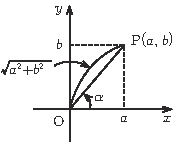
\includegraphics{./fig/sec00_5_1.pdf}}
三角関数 $ a\sin\theta+b\cos\theta$ は,点 $\mathrm{P}(a,\ b)$ を{\it xy}
座標平面にとり,$\mathrm{OP}=\sqrt{a^{2}+b^{2}}$ および $x$ 軸の正の向きか
ら $\overrightarrow{\mathrm{OP}}=(a,\ b)$ に向かって測った角 $\alpha$ に着目すると,
\end{Mw}
\begin{fleqn}[4zw]
\begin{alignat}{2}
&a\sin\theta+b\cos\theta\notag\\
=\;&\sqrt{a^2 + b^2}\left (\frac{a}{\sqrt{a^2 + b^2}}\sin\theta + \frac{b}{\sqrt{a^2 + b^2}}\cos\theta \right) \notag\\[3mm]
=\;&\sqrt{a^2 + b^2}(\cos\alpha\sin\theta + \sin\alpha\cos\theta) \notag\\[3mm]
=\;&\sqrt{a^2 + b^2}\sin(\theta + \alpha) \hspace{2zw} \left (\cos\alpha=\frac{a}{\sqrt{a^2 + b^2}}, \sin\alpha=\frac{b}{\sqrt{a^2 + b^2}} \right) \notag
\end{alignat}
\end{fleqn}

この公式を,三角関数の\textbf{合成公式}という.

\step{基本問題を解いてみよう}

\begin{例題}[1]
$x, y$ \text{の連立方程式}
\begin{fleqn}[4zw]
\[
\left\{\begin{array}{rl}
13\,\cos x+\sqrt{3}\sin x&=y\cos x\\
\sqrt{3}\,\cos x+1\mathrm{l}\sin x&=y\sin x
\end{array}\right.
\]
\end{fleqn}
の2組の解を$(x_{1}, y_{1})$,\ $(x_{2}, y_{2})$(ただし,$0\leqq x_{1}\leqq x_{2}<\pi$)とするとき,$x_{1}$, $y_{1}$, $x_{2}$, $y_{2}$の値を求めよ.
\end{例題}
\vspace{\baselineskip}

\begin{解答}

\vspace{-\baselineskip}\vspace{-\abovedisplayskip}
\begin{fleqn}[4zw]
%\vspace{-\baselineskip}\vspace{-\abovedisplayskip}
\hspace{4zw}$\left\{\begin{array}{rrr}
13\,\cos x+\sqrt{3}\sin x&=y\cos x & \hspace{13zw}{……①}\\
\sqrt{3}\,\cos x+11\sin x&=y\sin x & \hspace{13zw}{……②}
\end{array}\right.$
\end{fleqn}

$\Mframe{\text{①}\times\sin x-\text{②}\times\cos x}$\Footnote{連立方程式の未知数$x,y$のうち,簡単に消去できる$y$を消去.}より
\begin{fleqn}[4zw]
\begin{alignat*}{2}
&\sin x(13\cos x+\sqrt{3}\sin x)
-\cos x(\sqrt{3}\cos x+11\sin x)=0\notag\\
&\,2 \sin x\cos x- \sqrt{3}(\cos^{2}x-\sin^{2}x)=0\notag\\[-3pt]
&\sin 2x-\sqrt{3}\cos 2x=0\hspace{2zw}\therefore\hspace{1zw}\tan 2x=\frac{\sin 2x}{\cos 2x}=\sqrt{3}\notag
\end{alignat*}
\end{fleqn}

$ 0\leqq x<\pi$ のとき $ 0\leqq 2x<2\pi$ だから

\begin{fleqn}[4zw]
\begin{alignat*}{2}
&2x=\frac{\pi}{3},\ \frac{4}{3}\pi \qquad \therefore\quad x=\frac{\pi}{6},\ \frac{2}{3}\pi
\end{alignat*}
\end{fleqn}

①,②より,$ 0\leqq x_{1}<x_{2}<\pi$ だから

\begin{fleqn}[4zw]
\begin{alignat*}{2}
&x_{1}=\frac{\pi}{6},\, y_{1}=14,\, x_{2}=\frac{2}{3}\pi,\, y_{2}=10 \tag*{\kotae}
\end{alignat*}
\end{fleqn}
%\vspace{\baselineskip}
\end{解答}

\begin{例題}[2]
実数 $x, y$ が $x^{2}+4xy+5y^{2}-3=0$ を満たしている.このとき,$2x^{2}+xy+3y^{2}$のとりうる値の範囲を求めよ.
\end{例題}

\medskip
\begin{解答}
$2x^{2}+xy+3y^{2}=P$ とおくと
\begin{align*}
8x^{2}+4xy+12y^{2}\mathop{=}^{\text{\ajMaruKata{2}}}4P \tag*{……①}%\cdots\cdots\text{①}\\
\end{align*}
一方,条件式を
\[
x^{2}+4xy+5y^{2}=3\tag*{……②}
\]
とおく.① $-$ ②から,$7x^{2}+7y^{2}=4P-3$,すなわち
\[
7(x^{2}+y^{2})=4P-3\tag*{……③}
\]
\addtocounter{footnote}{1}
\footnotetext{条件式$x^2+4\,xy+5y^2=3$の$xy$の係数4に着目して,$4P$を考える.}\footnotetext[3]{2倍角および半角公式より.}\footnotetext[4]{合成公式より.}
ここで,極座標$(x,y)=(r\cos\theta,r\sin\theta)\ (r>0,\ 0\leqq\theta<2\pi)$
を用いて②上の点を表すと
\begin{fleqn}[4zw]
\begin{align}
(r\cos\theta)^{2}+4(r\cos\theta)(r\sin\theta)+5(r\sin\theta)^2=3\notag\\
(\cos^{2}\theta+4\sin\theta\cos\theta+5\sin^{2}\theta)r^{2}=3\notag
\end{align}
\end{fleqn}
よって,
\begin{alignat}{2}
r^{2}&=\frac{3}{\cos^{2}\theta+4\sin\theta\cos\theta+5\sin^{2}\theta}\notag\\
&\qerel{=}{3}\frac{3}{{\displaystyle \frac{1+\cos 2\theta}{2}}+2\sin 2\theta+5\cdot{\displaystyle \frac{1-\cos 2\theta}{2}}}\notag\\
&=\frac{3}{3+2(\sin 2\theta-\cos 2\theta)}\qerel{=}{4}\frac{3}{3+2\sqrt{2}\sin{\displaystyle \left (2\theta-\frac{\pi}{4}\right )}}\notag
\end{alignat}

$ 0\leqq\theta<2\pi$ のとき,$-1\leqq\sin\left (2\theta-\frac{\pi}{4}\right )\leqq 1$ だから

\begin{fleqn}[4zw]
\begin{alignat}{2}
&\frac{3}{3+2\sqrt{2}}\leqq r^{2}\leqq\frac{3}{3-2\sqrt{2}}\notag\\[3mm]
\therefore\hspace{1zw} &3 (3-2\sqrt{2})\leqq r^{2}\leqq 3(3+2\sqrt{2})\tag*{……④}
\end{alignat}
\end{fleqn}

③から,$7r^{2}=4P-3$ だから,\hspace{2zw}$P=\frac{7r^{2}+3}{4}$

よって,④から
\[
\frac{3(11-7\sqrt{2})}{2}\leqq P\leqq\frac{3(11+7\sqrt{2})}{2}\tag*{\kotae}
\]
%%%%%%%%赤字に従って、2Q落としています%%%%%%%%
\setcounter{footnote}{4}
{\footnotesize
\textbf{\fbox{参考}}\quad 条件式$\mathrm{C}_1: \, x^2+4xy+5y^2-3=0$も,
値の範囲を考えた$\mathrm{C}_2: \, 2x^2+xy+3y^2=P$もいずれも$x, \, y$についての2次式であり,
これらを満たす点$(x, \, y)$が描く図形は\Mframe{2次曲線}\footnote{2次曲線については,姉妹書『合格ナビ! 数学検定1級1次 線形代数』で詳しく学ぶ.ここでは2次曲線の描き方を既知として解説する.}である.
2次曲線には放物線や双曲線も含まれるが,本問の$\mathrm{C}_1, \, \mathrm{C}_2$はいずれも下図のような楕円である.
ここで楕円$\mathrm{C}_2$の$P$は定数とみなし,例として$P=5, 10$の場合を点線で描いた.
(容易に推測できると思うが,)$P$が大きくなると楕円$C_2$も大きくなる.

 さて本問は,点$(x, \, y)$が条件を満たしながら変化するとき,$P$の値がどのような範囲を動くかを求める問題であった.
言い換えると,
楕円$\mathrm{C}_1$と楕円$\mathrm{C}_2$が共有点をもつような範囲内で$P$が最大あるいは最小になるときを考えることにほかならない.
下図において$P$の値を変化させてみると,それはそれぞれ楕円$\mathrm{C}_2$が楕円$\mathrm{C}_1$に外接,内接するときであるとわかる.\VS{.5}
\begin{center}
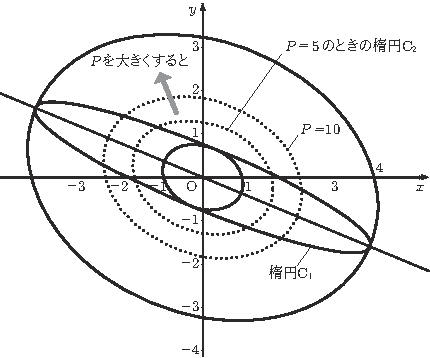
\includegraphics[scale=1]{./fig/sec00_betsu02.pdf}
\end{center}

\VS{.5}
また,\hspace{1zw}$P=\frac{3(11\pm 7\sqrt{2})}{2}$ のとき
\[
r^{2}=3(3\pm 2\sqrt{2}) \quad  \text{かつ} \quad  \sin\left(2\theta-\frac{\pi}{4}\right)=\mp 1\quad \text{(複号同順)}
\]\par}
%%%%%%%%%%%%%%%%%%%%%%%%%%%%%%%%%%%%%%%%%%%%%%
\end{解答}
\section{漸化式(1)}

\step{基本を確認しておこう}

数列 $\{a_{n}\}$ を隣りあったいくつかの項の間に成り立つ関係式で定義したものを,\textbf{数列の帰納的定義}といい,その関係式を数列の\textbf{漸化式}という.

\begin{titlebox}{等差数列,等比数列の帰納的定義}
\vskip1mm

\hspace{4zw}
$\begin{array}{l}
\text{等差数列:\ } a_{n+1}-a_n=d\hspace{1zw}(n \geqq 1,\ d\text{は定数})\\
\text{等比数列:\ } a_{n+1}=ra_n\hspace{1zw}(n \geqq 1,\ r\text{は定数})
\end{array}$\\
\vskip-.5mm
\end{titlebox}

漸化式の型(タイプ)によって,一般式への変形の方法は異なる.主なものを次に挙げる.

\begin{titlebox}{2項間の漸化式}
\vskip1mm
a.\hspace{1zw}
$a_{n+1}=a_n+f(n)\hspace{1zw}(n \geqq 1)\qquad(\text{階差型})$
\end{titlebox}
 この式の $n$ に$1, 2, \ldots, n-1$ を代入して,辺々加えると
\[
a_{n}=a_{\mathrm{1}}+\sum_{k=1}^{n-1}f(k)\hspace{1zw}(n\geqq 2)
\]

\begin{shadebox}
b.\hspace{1zw}$a_{n+1}=pa_n+q\hspace{2zw}(n \geqq 1,\ p \neq 0,1,\ q \neq 0)$
\end{shadebox}
 $a_{n},\ a_{n+1}$ を $t$ とおいて, $\Mframe{t=pt+q}$\Footnote{これを特性方程式という.} を解くと, $t=\frac{q}{1-p}$

\noindent
この $t$ の値を漸化式の両辺から引くと\hspace{1zw} $a_{n+1}-\frac{q}{1-p}=p\left (a_{n}-\frac{q}{1-p}\right )$\par
\noindent
$a_{n}-\frac{q}{1-p}=\left (a_{1}-\frac{q}{1-p}\right )p^{n-1}\hspace{2zw}\therefore\hspace{1zw}a_{n}=\frac{q}{1-p}+\left (a_{1}-\frac{q}{1-p}\right )p^{n-1}$
\begin{shadebox}
c.\hspace{1zw}$a_{n+1}=pa_n+f{(n)}\hspace{2zw}(n \geqq 1,\ p \neq 0,1)$
\end{shadebox}
 両辺を $p^{n+1}$ で割ると 

\[
\frac{a_{n+1}}{p^{n+1}}=\frac{a_{n}}{p^{n}}+\frac{f(n)}{p^{n+1}}=\frac{a_{n}}{p^{n}}+g(n)$\hspace{2zw}$\bigg (g(n)=\dfrac{f(n)}{p^{n+1}}$ とおく $\bigg )
\]

$\frac{a_{n}}{p^{n}}=b_{n}$ とおくと $b_{n+1}=b_{n}+g(n)$ となり,タイプa.に帰着する.\begin{shadebox}
d.\hspace{1zw}$a_{n+1}=\dfrac{pa_{n}+q}{ra_{n}+s} \quad (n \ge1, \, q \neq 0, \, r\neq 0, \, ps-qr\neq 0)$
\end{shadebox}
 $a_{n},a_{n+1}$を$t$とおいて,$t=\dfrac{pt+q}{rt+s}$ を解く.
整理すると$t$についての2次方程式$rt^{2}+(s-p)t-q=0 \, (r \neq 0)$となり,この特性方程式の2つの解を$\alpha, \beta$とする.

\noindent
(i) $\alpha \neq \beta$のとき;

漸化式の両辺から$\alpha$を引いて
\[
a_{n+1}-\alpha
=\dfrac{pa_{n}+q}{ra_{n}+s}-\alpha=\frac{(p-r\alpha)a_{n}+q-s\alpha}{ra_{n}+s}
\]
$r\alpha^{2}+(s-p)\alpha-q=0$から$q-s\alpha=-\alpha(p-r\alpha)$であるから
\begin{align}
a_{n+1}-\alpha
&=\dfrac{(p-r\alpha)(a_{n}-\alpha)}{ra_{n}+s} \\
\intertext{同様に,}
a_{n+1}-\beta
&=\dfrac{(p-r\beta)(a_{n}-\beta)}{ra_{n}+s}
\end{align}

①$\div$②から
$\dfrac{a_{n+1}-\alpha}{a_{n+1}-\beta}
=\dfrac{p-r\alpha}{p-r\beta} \cdot \dfrac{a_{n}-\alpha}{a_{n}-\beta}$

したがって,$\dfrac{a_{n}-\alpha}{a_{n}-\beta}=b_{n}$とおくと,
$b_{n+1}=\dfrac{p-r\alpha}{p-r\beta}b_{n}$となり,数列$\{ b_{n} \}$は等比数列となる.
これの一般式を求めれば,$\{ a_{n} \}$の一般式も得られる.

\noindent
(ii) 
$\alpha=\beta$のとき;

①,②は一致する.
①の両辺の逆数をとって$\dfrac{1}{a_{n}-\alpha}=c_{n}$とおくことにより,数列$\{ c_{n} \}$の漸化式にもち込む.

\step{基本問題を解いてみよう}
\begin{例題}
数列 $\{a_{n}\}$ において,次の関係があるとき,それぞれの一般項を求めよ.

\begin{Description}{2.5zw}
\item[(1)]
$a_{1}=2,\ a_{n}=a_{n-1}+n(n-1)\quad (n\geqq 2)$
\item[(2)]
$a_{1}=2,\ a_{n+1}=\frac{a_{n}}{a_{n}+3}\quad (n \geqq 1)$
\item[(3)]
$a_{1}=2,\ a_{n+1}=\frac{a_{n}+2}{2a_{n}+1}\quad (n\geqq 1)$
\end{Description}
\end{例題}

\begin{解答}
(1) 条件式から $a_{n+1}-a_{n}=n(n+1)$ で,$n\geqq 2$ のとき\footnotetext[2]{$a_n-a_{n-1}=n(n-1)$から$a_n=a_1+\sum_{k=1}^{n-1}k(k-1)$としてはいけない.}
\begin{align*}
%& \Mframe{a_{n}=a_{1}+\sum_{k=1}^{n-1}k(k+1)}\Footnotemark[2] \qerel{=}{2}2+\frac{1}{3}(n-1)n(n+1)\\
& \Mframe{a_{n}=a_{1}+\sum_{k=1}^{n-1}k(k+1)}\Footnotemark[2] \mathop{=}^{\text{\ajMaruKata{3}}}2+\frac{1}{3}(n-1)n(n+1)\\
&\hphantom{a=}=\frac{n^{3}-n+6}{3}=\frac{1}{3}(n+2)(n^{2}-2n+3)
\end{align*}
$a_{1}=2$ だから,この式は $n=1$ でも成り立つ.よって,\footnotetext[3]{$\sum_{k=1}^{n}k(k+1)=\frac{1}{3}n(n+1)(n+2)$を用いた.}
\begin{equation*}
a_{n}=\frac{1}{3}(n+2)(n^{2}-2n+3)\tag*{\kotae}
\end{equation*}

(2) 漸化式の両辺の逆数をとると
\begin{align*}
\frac{1}{a_{n+1}}=\frac{a_{n}+3}{a_{n}}=1+\frac{3}{a_{n}}
\end{align*}
$\frac{1}{a_{n}}=b_{n}$ とおくと\hspace{1zw}$b_{n+1}=3b_{n}+1$\vs{-2mm}
\begin{align*}
\Mframe{b_{n+1}+\frac{1}{2}=3\left (b_{n}+\frac{1}{2}\right )}\Footnotemark[4]
\end{align*}\footnotetext[4]{特性方程式$t=3t+1$を解いて$t=-\frac{1}{2}$}
したがって,数列 $\left\{b_{n}+\frac{1}{2}\right\}$ は初項 $b_{1}+\frac{1}{2}=\frac{1}{a_{1}}+\frac{1}{2}=1$,
公比が3の等比数列だから
\[
b_{n}+\frac{1}{2}=1\cdot 3^{n-1} \hspace{3zw} \therefore \hspace{1zw} b_{n}=\frac{2\cdot 3^{n-1}-1}{2}
\]
\begin{fleqn}
\begin{alignat}{1}
\text{よって,}\hspace{.5zw}a_{n}=\frac{1}{b_{n}}=\frac{2}{2\cdot 3^{n-1}-1}\tag*{\kotae}
\end{alignat}
\end{fleqn}

(3)\ 特性方程式 $t=\dfrac{t+2}{2t+1}$を解くと,$t^{2}=1$より$t=\pm1$.
これより
\begin{fleqn}[4zw]
\begin{alignat}{3}
&a_{n+1}-1&\;=\frac{a_{n}+2}{2a_{n}+1}-1=-\frac{a_{n}-1}{2a_{n}+1}\notag\\[3mm]
&a_{n+1}+1&\;=\frac{a_{n}+2}{2a_{n}+1}+1=\frac{3(a_{n}+1)}{2a_{n}+1}\notag
\end{alignat}
\end{fleqn}
\text{したがって,}\ $\frac{a_{n+1}-1}{a_{n+1}+1}=-\frac{1}{3}\cdot\frac{a_{n}-1}{a_{n}+1}$

$b_{n}=\frac{a_{n}-1}{a_{n}+1}$ とおくと\hspace{.5zw} $b_{n+1}=-\frac{1}{3}b_{n}$

$b_{1}=\frac{a_{1}-1}{a_{1}+1}=\frac{1}{3}$ より\hspace{.5zw} $b_{n}=\frac{1}{3}\left (-\frac{1}{3}\right )^{n-1}=-\left (-\frac{1}{3}\right )^{n}$

\begin{fleqn}
\begin{alignat}{1}
よって,a_{n}\qerel{=}{5}\frac{1+b_{n}}{1-b_{n}}=\frac{1-\left (-\frac{1}{3}\right )^{n}}{1+\left (-\frac{1}{3}\right )^{n}}=\frac{3^{n}-\left (-1\right )^{n}}{3^{n}+(-1)^{n}}\tag*{\kotae}
\end{alignat}\footnotetext[5]{$(a_n+1)b_n=a_n-1$を$a_n$について整理した.}
\end{fleqn}


\end{解答}

\section{漸化式(2)}
\step{基本を確認しておこう}

\begin{titlebox}{3項間の漸化式}
$\hspace{4zw}a_{n+2}=pa_{n+1}+qa_{n}\, (p\neq 0,\ q\neq 0)$
\end{titlebox}
漸化式の $a_{n+2},\ a_{n+1},\ a_n$をそれぞれ $t^{2}, t, 1$におきかえた $t$ の2次方程式 $t^{2}-pt-q=0$を考える.この特性方程式の2解を $\alpha,\ \beta$ とすると,解と係数の関係から
$
\alpha+\beta=p,\ \alpha\beta=-q
$であり,一般項 $a_{n}$ は次のいずれかの形になる.

\begin{fleqn}[4zw]
\[
\begin{array}{r@{\ }l}
\text{(i)}&\alpha\neq\beta\text{のとき,\null}a_{n}=A\cdot\alpha^{n-1}+B\cdot\beta^{n-1}\\[1mm]
\text{(ii)}&\alpha=\beta\text{のとき,\null}a_{n}=(An+B)\cdot\alpha^{n-1}
\end{array}(A,\ B\ \text{は定数})
\]
\end{fleqn}

\begin{zDescription}
\item[\hbox{(i)}] $\alpha\neq\beta$ のとき
\begin{align*}
a_{n+2}-\alpha a_{n+1}&=pa_{n+1}+qa_{n}-\alpha a_{n+1}=(p-\alpha)a_{n+1}+qa_{n}\\
&=\beta a_{n+1}-\alpha\beta a_{n}=\beta(a_{n+1}-\alpha a_{n})
\end{align*}
\begin{fleqn}[0zw]
\begin{alignat}{2}
\text{これより,}\ & a_{n+1}-\alpha a_{n}=(a_{2}-\alpha a_{1})\beta^{n-1}\tag*{……①}\\%
\mbox{同様に,}\hspace{1.3zw} & a_{n+1}-\beta a_{n}=(a_{2}-\beta a_{1})\alpha^{n-1}\tag*{……②}
\end{alignat}
\end{fleqn}
$\text{①}-\text{②}$から,$(\beta-\alpha)a_{n}=(a_{2}-\alpha a_{1})\beta^{n-1}-(a_{2}-\beta a_{1})\alpha^{n-1}$\\
よって,$a_{n}=\frac{1}{\beta-\alpha}\{(a_{2}-\alpha a_{1})\beta^{n-1}-(a_{2}-\beta a_{1})\alpha^{n-1}\}$

\item[\hbox{(ii)}]
$ \alpha=\beta$ のとき\par
①,②は一致し,$a_{n+1}-\alpha a_{n}=(a_{2}-\alpha a_{1})\alpha^{n-1}$ となるので,両辺を $\alpha^{n+1} (\neq 0)$ で割ることにより $a_{n}$ を求めることができる.
\end{zDescription}

\begin{titlebox}{連立漸化式}
\[\left\{\begin{array}{l}
a_{n+1}=pa_{n}+qb_{n}\\
b_{n+1}=ra_{n}+sb_{n}
\end{array}\right.\]
\end{titlebox}
$\{a_{n}\}$ だけについての3項間の漸化式を導くと,次のようになる.

\begin{fleqn}[4zw]
\begin{alignat}{2}
a_{n+2}&=pa_{n+1}+qb_{n+1}=pa_{n+1}+q(ra_{n}+sb_{n})\notag\\
&=pa_{n+1}+qra_{n}+s(a_{n+1}-pa_{n})=(p+s)a_{n+1}-(ps-qr)a_{n}\notag
\end{alignat}
\end{fleqn}
あるいは,数列 $\{a_{n}+\alpha b_{n}\}$ が公比 $\beta$ の等比数列になるように考えてもよい.

\noindent
$a_{n+1}+\alpha b_{n+1}=\beta(a_{n}+\alpha b_{n}) \text{から}$
\begin{fleqn}[4zw]
\begin{alignat}{2}
(pa_{n}+qb_{n})+\alpha(ra_{n}+sb_{n})&=\beta(a_{n}+\alpha b_{n})\notag\\
(p+\alpha r)a_{n}+(q+\alpha s)b_{n}&=\beta a_{n}+\alpha\beta b_{n}\notag
\end{alignat}
\end{fleqn}
これより,$ p+\alpha r=\beta$ かつ $ q+\alpha s=\alpha\beta$ から $\alpha, \beta$ の値を求める.

\step{基本問題を解いてみよう}

\begin{例題}
%\vspace{-\baselineskip}\vspace{-\abovedisplayskip}
\begin{fleqn}[4zw]
(1)\ 数列 $\{a_{n}\}$ が $a_{n+2}=4a_{n+1}-4a_{n}\,(n\geqq 1) , a_{1}=1, a_{2}=8$で定義されるとき,一般項 $a_{n}$ を求めよ.\par
\noindent
(2)\ 2つの数列 $\{x_{n}\}, \{y_{n}\}$ が関係式
\[
x_{1}=11,\quad y_{1}=1,\quad x_{n+1}=6x_{n}+5y_{n},\quad y_{n+1}=x_{n}+2y_{n}\,(n\geqq 1)
\]
で定められるとき,一般項 $x_{n}, y_{n}$ を求めよ.
\end{fleqn}
\end{例題}

\medskip
\begin{解答}
%\vspace{-\baselineskip}\vspace{-\abovedisplayskip}
(1)\ 特性方程式$t^{2}-4t+4=0$ を解くと,$(t-2)^{2}=0$より
$t=2$(2 \text{重解}).

\begin{fleqn}[4zw]
これより,$a_{n+2}-2a_{n+1}=2(a_{n+1}-2a_{n})$

したがって,数列 $\{a_{n+1}-2a_{n}\}$ は初項 $a_{2}-2a_{1}=8-2\cdot 1=6$,公比2の等比数列だから
\begin{align*}
a_{n+1}-2a_{n}=6\cdot 2^{n-1}=3\cdot 2^{n}
\end{align*}
両辺を $2^{n+1}$ で割ると
$\Mframe{\frac{a_{n+1}}{2^{n+1}}-\frac{a_{n}}{2^{n}}=\frac{3}{2}}
\Footnote{$\frac{a_n}{2^n}=b_n$とおくと$b_{n+1}-b_{n}=\frac{3}{2}$(=一定)}$\\
数列 $\left\{\frac{a_{n}}{2^{n}}\right\}$ は初項 $\frac{a_{1}}{2^{1}}=\frac{1}{2}$,公差 $\frac{3}{2}$ の等差数列だから,
\[
\frac{a_{n}}{2^{n}}=\frac{1}{2}+(n-1)\cdot\frac{3}{2}=\frac{3n-2}{2}
\]

\end{fleqn}
\begin{fleqn}

\noindent
\begin{align*}
\text{よって,}\hspace{.5zw}a_{n}=(3n-2)\cdot 2^{n-1}\tag*{\kotae}
\end{align*}

\end{fleqn}
\begin{fleqn}[4zw]

(2) \hspace{1zw} $x_{n+1}=6x_{n}+5y_{n},y_{n+1}=x_{n}+2y_{n}$

$y_n$を消去して $x_{n}$ だけの漸化式を導くと
\begin{alignat}{2}
x_{n+2}&=6x_{n+1}+5y_{n+1}=6x_{n+1}+5(x_{n}+2y_{n})\notag\\
&=6x_{n+1}+5x_{n}+2(x_{n+1}-6x_{n})=8x_{n+1}-7x_{n}\notag
\end{alignat}
すなわち,$x_{n+2}=8x_{n+1}-7x_{n}$\\
特性方程式$t^2=8t-7$を解いて,$t=1,7$

これを用いて変形すると,
\begin{alignat}{3}
& x_{n+2}-x_{n+1}&&=7(x_{n+1}-x_{n})\tag*{……①}\\
& x_{n+2}-7x_{n+1}&&=x_{n+1}-7x_{n}\tag*{……②}
\end{alignat}
\end{fleqn}
\begin{fleqn}[4zw]
①から,数列 $\{x_{n+1}-x_{n}\}$ は初項 $x_{2}-x_{1}=71-11=60$,公比7の等比数列だから
\begin{alignat*}{1}
x_{n+1}-x_{n}=60\cdot 7^{n-1}\tag*{……③}
\end{alignat*}
②から,数列 $\{x_{n+1}-7x_{n}\}$ は初項 $x_{2}-7x_{1}=71-77=-6$ の定数数列だから
\begin{alignat*}{1}
x_{n+1}-7x_{n}=-6 \tag*{……④}
\end{alignat*}
$\text{③}-\text{④}$から $6x_{n}=60\cdot 7^{n-1}+6$.よって,
$x_{n}=10\cdot 7^{n-1}+1 $

関係式より
\begin{alignat*}{1}
5y_{n}&=x_{n+1}-6x_{n}\notag\\
&=(10\cdot 7^{n}+1)-6(10\cdot 7^{n-1}+1)=10\cdot 7^{n-1}-5\notag
\end{alignat*}

よって,$y_{n}=2\cdot 7^{n-1}-1$

以上より,
\[
x_n=10\cdot7^{n-1}+1,\qquad y_n=2\cdot7^{n-1}-1\tag*{\kotae}
\]
\end{fleqn}
\end{解答}

\section{二項定理}
\step{基本を確認しておこう}


\begin{titlebox}{二項定理}
任意の自然数 $n$ に対して,
\begin{fleqn}[1zw]
\begin{alignat*}{2}
(a+b)^n &= \sum_{r=0}^{n}\,{}_{n}\!\mathrm{C}_{r}a^{n-r}b^r\\
&={}_{n}\!\mathrm{C}_{0}a^n+{}_{n}\!\mathrm{C}_{1}a^{n-1}b+\cdots
+{}_{n}\!\mathrm{C}_{r}a^{n-r}b^r+\cdots+{}_{n}\!\mathrm{C}_{n}b^n\notag
\end{alignat*}
\end{fleqn}
\end{titlebox}

展開式の各項の係数${}_{n}\!\mathrm{C}_{r}\,(r=0,1,2,\ldots,\ n)$ を二項係数という.${}_{n}\!\mathrm{C}_{r}$を$\Binom{n}{r}$と書くこともある.これは $n$ 個のものから $r$ 個をとる組合せの数に等しい.また,展開式における $(r+1)$ 番目の項 ${}_{n}\!\mathrm{C}_{r}a^{n-r}b^{r}$ を,$(a+b)^{n}$ の展開式の\textbf{一般項}という.特に,
\begin{fleqn}[2zw]
\begin{equation}
(1+x)^{n}=\sum_{r=0}^{n}{}_{n}\!\mathrm{C}_{r}x^{r}={}_{n}\!\mathrm{C}_{0}+{}_{n}\!\mathrm{C}_{1}x+{}_{n}\!\mathrm{C}_{2}x^{2}+\cdots+{}_{n}\!\mathrm{C}_{n}x^{n}\tag*{……①}
\end{equation}
\end{fleqn}

\noindent
からは,いろいろな有用な等式を導くことができる.\par
\noindent
$x=1$ とおくと ${}_{n}\!\mathrm{C}_{0}+{}_{n}\!\mathrm{C}_{1}+{}_{n}\!\mathrm{C}_{2}+\cdots+{}_{n}\!\mathrm{C}_{n}=2^{n}$\par
\noindent
$x=-1$ とおくと ${}_{n}\!\mathrm{C}_{0}-{}_{n}\!\mathrm{C}_{1}+{}_{n}\!\mathrm{C}_{2}-\cdots+(-1)^{n}{}_{n}\!\mathrm{C}_{n}=0$

\noindent
①の両辺を $x$ で微分して
\begin{fleqn}[4zw]
\begin{alignat*}{1}
n(1+x)^{n-1}={}_{n}\!\mathrm{C}_{1}+2 {}_{n}\!\mathrm{C}_2x+3{}_{n}\!\mathrm{C}_{3}x^{2}+\cdots+n{}_{n}\!\mathrm{C}_{n}x^{n-1}
\end{alignat*}
\end{fleqn}\par
\noindent
$x=1$ とおくと ${}_{n}\!\mathrm{C}_{1}+2{}_{n}\!\mathrm{C}_{2}+3{}_{n}\!\mathrm{C}_{3}+ \cdots +n_{n}\!\mathrm{C}_{n}=n\cdot 2^{n-1}$

\step{基本問題を解いてみよう}
\begin{例題}
(1) \quad $\frac{1\cdot {}_{10}\mathrm{C}_{1}+2\cdot {}_{10}\mathrm{C}_{2}+3\cdot {}_{10}\mathrm{C}_{3}+\cdots+10\cdot {}_{10}\mathrm{C}_{10}}{{}_{10}\mathrm{C}_{0}+{}_{10}\mathrm{C}_{1}+{}_{10}\mathrm{C}_{2}+\cdots+_{10}\!\mathrm{C}_{10}}$ の値を求めよ.
(2) \quad $\sum_{k=1}^{n}(x+2)^{k}$ を展開したときの $x$ の係数を求めよ.
\end{例題}

\begin{解答}
(1) \hspace{.5zw} $k$ が自然数のとき

\begin{fleqn}[4zw]
\[
k\cdot {}_{10}\mathrm{C}_{k}=k\cdot\frac{10!}{k!(10-k)!}
=\frac{10\cdot 9!}{(k-1)!\{9-(k-1)\}!}=10\cdot {}_{9}\mathrm{C}_{k-1}
\]
\begin{alignat*}{2}
\text{分子} &=\sum_{k=1}^{10}k\cdot_{10}\mathrm{C}_{k}=\sum_{k=1}^{10}10\cdot {}_{9}\mathrm{C}_{k-1}\notag\\[3mm]
&=10({}_{9}\mathrm{C}_{0}+{}_{9}\mathrm{C}_{1}+{}_{9}\mathrm{C}_{2}+\cdots+{}_{9}\mathrm{C}_{9})\notag\\
&=10(1+1)^{9}=10\cdot 2^{9}=5\cdot 2^{10}
\end{alignat*}
$\text{また,分母} =(1+1)^{10}=2^{10}$\\
$\text{よって,与式} =\frac{5\cdot 2^{10}}{2^{10}}=5$\hfill{\kotae}

\noindent
(2)\hspace{1zw}$(x+2)^{k}={}_{k}\mathrm{C}_{0}\cdot 2^{k}+{}_{k}\mathrm{C}_{1}\cdot 2^{k-1}x+{}_{k}\mathrm{C}_{2}\cdot 2^{k-2}x^{2}+\cdots+_{k}\!\mathrm{C}_{k}x^{k}$
\end{fleqn}

\hspace*{1zw}%
$\sum_{k=1}^{n}(x+2)^{k}$ の展開式における $x$ の係数は,
\begin{fleqn}[4zw]
\[
\sum_{k=1}^{n}{}_{k}\mathrm{C}_{1}\cdot 2^{k-1}=\sum_{k=1}^{n} k\cdot 2^{k-1}\,(\Mframe{=S_nとおく}\Footnotemark[1])
\]
\addtocounter{footnote}{1}
\footnotetext[1]{$S_{n}= \displaystyle \sum_{k=1}^{n} k \cdot r^{k-1} \, (r \neq 0, \, 1)$は$S_{n}-rS_{n}$を考えることにより求める.
}
\end{fleqn}

%%%%%%差し替え前%%%%%%
%\hspace*{1zw}%
%$k\cdot 2^{k-1}=(k-1)\cdot 2^{k}-(k-2)\cdot 2^{k-1}$ だから
%\begin{fleqn}[4zw]
%\begin{alignat*}{2}
%S_{n}&=\sum_{k=1}^{n}\{(k-1)\cdot 2^{k}-(k-2)\cdot 2^{k-1}\}\notag\\[3mm]
%&=(n-1)\cdot 2^{n}+1\tag*{\kotae}
%\end{alignat*}
%\end{fleqn}

\begin{center}
$
\begin{array}{lcllrl}
 S_{n}&=&1+2 \cdot & 2+3 \cdot 2^{2}+\cdots &+n     \cdot 2^{n-1}& \\
2S_{n}&=&          & 2+2 \cdot 2^{2}+\cdots &+(n-1) \cdot 2^{n-1}& +n \cdot 2^{n}
\end{array}$
\end{center}
辺々を引くと,
\begin{align*}
-S_{n}&=1+2+2^{2}+\cdots+2^{n-1}-n \cdot 2^{n} \\
      &=\dfrac{2^{n}-1}{2-1}-n \cdot 2^{n}
       =-(n-1) \cdot 2^{n}-1
\end{align*}
よって,求める$x$の係数は
\[
S_{n}=(n-1)\cdot2^{n}+1 \hfill\text{……(答)}
\]
\end{解答}
\step{過去問題にチャレンジ!}
\begin{問題}[1]
 次の連立方程式を複素数の範囲で解きなさい.
\[
\left\{\begin{array}{l}
 x^{3}+xy+y^{3}=11 \\ 
 x^{3}-xy+y^{3}=7
\end{array}\right.
\]
\end{問題}
\begin{解答}
\[
\left\{\begin{array}{l}
 x^{3}+xy+y^{3}=11 \\ 
 x^{3}-xy+y^{3}=7
 \end{array}\right.
	\tag*{$\begin{array}{r@{}}
	{……①}\\
	{……②}\end{array}$%
	}%
\]
とする.

①+②より${2}x^{3}+2y^{3}=18$,すなわち$x^{3}+y^{3}=9$\,\hfill{……③}

(①-②)$\div 2$より$xy=2$,すなわち$x^{3}y^{3}=8$\,\hfill{……④}

③,④より$x^{3},\,y^{3}\!$を解にもつ2次方程式は${t}^{2}-9t+8=0$

これを解くと $t=1,8$

よって$(x^{3},y^{3})=(1,8)$,$(8,1)$

$(x^{3},y^{3})=(1,8)$のとき,連立方程式 $x^{3}=1,\, xy=2$ を解いて
\[
(x,y)=(1,2),\left( \frac{-1\pm \sqrt 3 
i}{2},-1\mp \sqrt 3 i \right)\qquad\text{(複号同順)}
\]

$(x^{3},y^{3})=(8,1)$のとき,連立方程式 $x^{3}=8,\, xy=2$ を解いて
\[
(x,y)=(2,1),\left( -1\pm \sqrt{3}i,\frac{-1\mp 
\sqrt{3} i}{2} \right)\qquad\text{(複号同順)}
\]
 
以上より

$
(x,y)=(1,2),(2,1),\left(\frac{{-1\pm }\sqrt 
{3}{i}}{2}{,-1\mp }\sqrt {3} 
{i} \right),\left( {-1\pm }\sqrt {3} 
{i,}\frac{{-1\mp }\sqrt {3} {i}}{2} 
\right)\\\hfill\text{(複号同順)}{\kotae}
$

\end{解答}

\begin{解説}
次を利用して,まず $x^{3},\,y^{3}\!$の値を求める.

\textbf{解と係数の関係}\quad 2次方程式$ax^{2}+bx+c=0$\, 
の2つの解を\,$\alpha ,\beta $\, とするとき
\[
\alpha +\beta =-\frac{b}{a}\text{,}\ \alpha \beta 
=\frac{c}{a}
\]
\end{解説}
\begin{問題}[2]
$(1+x)^{n}$ の展開式を $c_{0}+c_{1}x+\cdots +c_{n}x^{n}$ とするとき,次の値を求めなさい.
\[
\sum\limits_{k=0}^n (-1)^{k}\frac{c_{k}}{k+1} 
\]
\end{問題}

\begin{解答}二項係数を$\Binom{n}{k}\left(=\dfrac{n!}{k!(n-k)!}\right)$で表すと
\begin{fleqn}[4zw]
\begin{alignat*}{2}
&\sum\limits_{k=0}^n (-1)^{k}\frac{c_{k}}{k+1} =\sum\limits_{k=0}^n \frac{(-1)^{k}}{k+1} \Binom{n}{k}\\
=&\sum\limits_{k=0}^n {\frac{(-1)^{k}}{k+1}\times \frac{k+1}{n+1}} 
\Binom{n+1}{k+1}=\, 
-\frac{1}{n+1}\sum\limits_{k=0}^n {\Binom{n+1}{k+1} 
\left( -1 \right)^{k+1}}\\
=&\, -\frac{1}{n+1}\left\{ \Binom{n+1}{0}+\sum\limits_{k=0}^n {\Binom{{n+1}}{{k+1}}
\left( -1 \right)^{k+1}-\Binom{n+1}{0}} 
\right\}\tag*{……①} 
\end{alignat*}
\end{fleqn}

ここで

\begin{fleqn}[4zw]
\begin{align*}
{(1+x)}^{n+1}&=\sum\limits_{k=0}^{n+1} \Binom{n+1}{k} 
 x^{k}=\, \Binom{n+1}{0}+\sum\limits_{k=1}^{n+1} 
{\Binom{n+1}{k}x^{k}}\\
 &=\, \Binom{n+1}{0}+\sum\limits_{k=0}^n {\Binom{n+1}{k+1}x^{k+1}}
\end{align*}
\end{fleqn}

に$x=-1$を代入して

\[
0=\Binom{n+1}{0}+\sum\limits_{k=0}^n \Binom{n+1}{k+1}
\left( -1 \right)^{k+1}
\]
 よって
\[
\text{①}=-\frac{1}{n+1}\times \left\{ -\Binom{n+1}{0}
\right\}=\frac{1}{n+1}\tag*{\kotae}
\]
\end{解答}

\begin{解説}
 次に示す\textbf{二項定理}を用いる.

\begin{fleqn}[4zw]
\begin{alignat*}{2}
(x+y)^{n}=&\sum\limits_{k=0}^n {c_{k}x^{k}y^{n-k}} \quad \left( 
c_{k}=\Binom{n}{k}=\frac{n!}{k!\left( n-k \right)!} \right) \\ 
&\text{(}\Binom{n}{k}\text{を\textbf{二項係数}という)}
\end{alignat*}

 二項係数について,次が成り立つ.
\[
\Binom{n}{k} = \frac{k+1}{n+1}\Binom{n+1}{k+1}
\]
\end{fleqn}
\end{解説}

% !TEX root = V:\暫定進行\tosyo\合格ナビ数検1級\解析編\main.tex
% !TEX program = uplatex
\chapter{極限}
\section{数列の極限}
\step{基本を確認しておこう}
無限数列$\{a_n\}$において,$n$が限りなく大きくなるとき,その極限は次のいずれかになる.
\begin{Description}{2.5zw}
\item[\hskip1zw a.]
収束 \hskip2zw$  \lim_{n \to \infty} a_n = \alpha \hspace{1zw}(一定の値\,\alpha\, に収束) $
\item[\hskip1zw b.]
発散\hskip2zw $\begin{cases}
{\displaystyle \lim_{n \to \infty}} a_n = \infty & (正の無限大に発散)\\[0.4zh]
{\displaystyle \lim_{n \to \infty}} a_n = -\infty & (負の無限大に発散)\\[0.4zh]
振動& (極限はない)
\end{cases}$
\end{Description}

\begin{titlebox}{数列の極限値の性質}
数列$\{a_n\},\{b_n\}$が収束し,$\displaystyle \lim_{n \to \infty} a_n = \alpha,\displaystyle \lim_{n \to \infty} b_n = \beta$であるとき
\begin{Description}{1.5zw}
\item[a.]$\displaystyle \lim_{n \to \infty} ca_n = c\alpha$($c$は定数)
\item[b.]$\displaystyle \lim_{n \to \infty} (a_n \pm b_n) = \alpha \pm \beta$(複号同順)
\item[c.]$\displaystyle \lim_{n \to \infty} a_nb_n = \alpha\beta$
\hskip26mm d.\hskip.5zw $\displaystyle \lim_{n \to \infty} \frac{a_n}{b_n} = \frac{\alpha}{\beta}$($\beta\neq0$)
\end{Description}
\end{titlebox}
さらに,数列の極限と大小関係については,次の性質が成り立つ.
\begin{itemize}
\item 数列$\{a_n\},\{b_n\}$において,$a_n\leqq b_n\,(n=1,2,3,\ldots)$のとき
\[\displaystyle \lim_{n \to \infty} a_n = \alpha,\displaystyle \lim_{n \to \infty} b_n = \beta \Longrightarrow \alpha\leqq \beta\]
\item 数列$\{a_n\},\{b_n\}$において,$a_n\leqq b_n\,(n=1,2,3,\ldots)$のとき
\[\displaystyle \lim_{n \to \infty} a_n = \infty \Longrightarrow \displaystyle \lim_{n \to \infty} b_n = \infty\]
\end{itemize}
\begin{titlebox}{はさみうちの原理}
数列$\{a_n\},\{b_n\},\{c_n\}$において,$a_n\leqq b_n\leqq c_n\,(n=1,2,3,\ldots)$のとき
\[\displaystyle \lim_{n \to \infty} a_n = \displaystyle \lim_{n \to \infty} c_n = \alpha \Longrightarrow \{b_n\} は収束して\displaystyle \lim_{n \to \infty} b_n = \alpha\]
\end{titlebox}
重要な無限数列についてまとめておこう.
\begin{Description}{2.5zw}
\item[\hskip1zw a.] $\displaystyle \lim_{n \to \infty} n^k\,(k \neq 0)$
\[ \displaystyle \lim_{n \to \infty} n^k = 
\Bigg\{\begin{array}{cl}
\infty & (k > 0)\\
0 & (k < 0)
\end{array}\]
\item[\hskip1zw b.] {無限等比数列} $\displaystyle \lim_{n \to \infty} r^n $
\[ \displaystyle \lim_{n \to \infty} r^n = 
\begin{cases}
\infty & (r > 1)\\
1 & (r = 1)\\
0 & (|r| < 1)\\
振動(極限はない) & (r \leqq -1)
\end{cases} \]
\item[\hskip1zw c.] $\displaystyle \lim_{n \to \infty} nr^n $
\[ \displaystyle \lim_{n \to \infty} nr^n = 
\begin{cases}
\infty & (r \geqq 1)\\
0 & (|r| < 1)\\
振動(極限はない) & (r \leqq -1)
\end{cases} \]
\end{Description}

\step{基本問題を解いてみよう}
\begin{例題}
次の極限を調べよ.
\begin{longtable}[l]{@{\hskip0zw}cl@{\hskip5zw}cl}
(1) & $\displaystyle \lim_{n \to \infty} \frac{-3{n^2} + 8}{5{n^2} - 3n + 1} $ & (2) & $\displaystyle \lim_{n \to \infty} \frac{2 - n}{3 + \sqrt{n}} $ \\[2zh]
(3) & $\displaystyle \lim_{n \to \infty} \frac{(-4)^n - 3}{2^n + 1} $ & (4) & $\displaystyle \lim_{n \to \infty} \frac{\sin 3n}{n} $
\end{longtable}
\end{例題}

\VS{-.75}
\begin{解答}
$\dis\begin{array}[t]{@{}l@{\hskip1zw}>{\dis}l>{\dis}c>{\dis}l}
(1) & \Mframe{\lim_{n \to \infty} \dfrac{-3{n^2} + 8}{5{n^2} - 3n + 1}}\Footnote{} &=& \lim_{n \to \infty} \dfrac{-3 + \dfrac{8}{n^2}}{5 - {\dfrac{3}{n}} + {\dfrac{1}{n^2}}}= -\dfrac{3}{5}
\end{array}$\footnotetext[1]{$\frac{\infty}{\infty}$の極限$\Longrightarrow$分母の最高次の項で分子・分母を割る.}\hfill\raisebox{0mm}{\Kotae}\par
$\dis\begin{array}[b]{@{}l@{\hskip1zw}>{\dis}l>{\dis}c>{\dis}l}
(2) & \lim_{n \to \infty} \dfrac{2 - n}{3 + \sqrt{n}} &=& \Mframe{\lim_{n \to \infty} \dfrac{\dfrac{2}{\sqrt{n}} - \sqrt{n}}{\dfrac{3}{\sqrt{n}} + 1}}\Footnote{}
= -\infty 
\end{array}$\footnotetext[2]{$n\to\infty$のとき,分子$\to-\infty$,分母$\to1$.}\kotae\par
$\dis\begin{array}[b]{@{}l@{\hskip1zw}>{\dis}l>{\dis}c>{\dis}l}
(3) & \lim_{n \to \infty} \dfrac{(-4)^n - 3}{{2^n} + 1} &=& \Mframe{\lim_{n \to \infty}\dfrac{(-2)^n - 3\left(\dfrac{1}{2}\right)^n}{1 + \left(\dfrac{1}{2}\right)^n}}\Footnote{}
\end{array}\\
よって,振動する
$\footnotetext[3]{$n\to\infty$のとき$\left(\frac{1}{2}\right)^n\!\!\to0,\ (-2)^n$は振動.}\kotae\par
$\dis\begin{array}[b]{@{}r@{\hskip1zw}>{\dis}l>{\dis}c>{\dis}l}
(4) &|\sin 3n| &\leqq& 1 であるから\hskip1zw
-\dfrac{1}{n}\leqq \dfrac{\sin 3n}{n} \leqq \dfrac{1}{n}
\end{array}$\\
$\begin{array}{@{}lcl}
\lim_{n \to \infty} \dfrac{1}{n} &=& \displaystyle \lim_{n \to \infty} \left ( - \dfrac{1}{n} \right ) = 0 であるから\\[1zh]
&&\lim_{n \to \infty} \dfrac{\sin 3n}{n}=0\footnotemark[4]
\end{array}$\footnotetext[4]{はさみうちの原理.} \kotae
\end{解答}
\section{無限級数}
\step{基本を確認しておこう}
無限数列$\{a_n\}$の各項を,記号$+$で結んだもの\pagebreak[3]
\[
a_1 + a_2 + a_3 + \cdots + a_n + \cdots
\]
を\textbf{無限級数}(または単に級数)といい,$\displaystyle \sum_{n=1}^\infty a_n$または$\displaystyle \sum a_n$と書く.
\[
S_n = \sum_{k=1}^n a_k = a_1 + a_2 + a_3 + \cdots + a_n 
\]
を無限級数$\displaystyle \sum_{n=1}^\infty a_n$の第$n$部分和という.
\begin{titlebox}{無限級数の収束・発散}
$\displaystyle \lim_{n \to \infty}S_n = \alpha$(有限確定値)のとき,無限級数$\displaystyle \sum_{n=1}^\infty a_n$は収束し,$\displaystyle \sum_{n=1}^\infty a_n = \alpha$と書く.収束しない級数は発散するという.
\end{titlebox}

2つの無限級数$\displaystyle \sum_{n=1}^\infty a_n,\sum_{n=1}^\infty b_n$がともに収束し,和がそれぞれ$\alpha,\,\beta$であるとき,定数$p,\,q$について
\[
\sum_{n=1}^\infty(pa_n + qb_n) = p\sum_{n=1}^\infty{a_n} + q\sum_{n=1}^\infty{b_n} = p\alpha + q\beta\,(収束)
\]
また,次は無限級数の収束・発散について重要である.
\begin{kakomi}
\begin{Description}{1.5zw}
\item[$\bullet$]
$\displaystyle \sum_{n=1}^\infty a_n$が収束する$\Longrightarrow \displaystyle\lim_{n \to \infty}a_n = 0$(収束するための必要条件)
\item[$\bullet$]$\displaystyle\lim_{n \to \infty}a_n \neq 0 \Longrightarrow \sum_{n=1}^\infty a_n$は発散する
\end{Description}
\end{kakomi}
特に,無限等比数列$\{ar^{n-1}\}$からつくられた無限級数
\[
\displaystyle \sum_{n=1}^\infty ar^{n-1} = a + ar + ar^2 + \cdots + \cdots
\]
を初項$a$,公比$r$の\textbf{無限等比級数}という.
\begin{titlebox}{無限等比級数の収束・発散}
$\displaystyle \sum_{n=1}^\infty ar^{n-1}$\,$(a \neq 0)$は,
\begin{Description}{1.5zw}
\item[$\bullet$]
$|r|<1$のとき収束して,$\displaystyle \sum_{n=1}^\infty ar^{n-1}= \frac{a}{1-r}$
\item[$\bullet$]
$|r|\geqq 1$のとき発散する
\end{Description}
\end{titlebox}

\step{基本問題を解いてみよう}
\begin{例題}
次の級数の収束・発散を調べ,収束するものについては和を求めよ.
\begin{longtable}[l]{@{\hskip0zw}cl@{\hskip5zw}cl}
(1) & $\displaystyle \sum_{n=1}^\infty \frac{1}{(3n - 1)(3n + 2)}$ & (2) & $\displaystyle \sum_{n=1}^\infty \left ( -\frac{1}{2} \right )^{2n-1} $ \\[2zh]
(3) & $\displaystyle \sum_{n=1}^\infty \frac{n}{2^{n-1}}$ & (4) & $\displaystyle \sum_{n=1}^\infty \frac{n}{2n + 1} $
\end{longtable}
\end{例題}\par
\begin{解答}
(1)\hskip1zw  $\dis\frac{1}{(3n - 1)(3n + 2)} \mathop{=}^{\text{\ajMaruKata{1}}} \frac{1}{3} \left (\frac{1}{3n - 1} - \frac{1}{3n + 2} \right )$であるから\footnotetext[1]{部分分数へ分解した.}
\begin{align*}
  S_n &= \frac{1}{3}\bigg \{ \left ( \frac{1}{2} - \frac{1}{5} \right ) + \left ( \frac{1}{5} - \frac{1}{8} \right ) + \left ( \frac{1}{8} - \frac{1}{11} \right ) \\[1zh]
&\quad  +\cdots + \left ( \frac{1}{3n - 1} - \frac{1}{3n + 2} \right ) \bigg \}\\[1zh]
&=\frac{1}{3}\left ( \frac{1}{2} - \frac{1}{3n + 2} \right )
\end{align*}
\[\lim_{n \to \infty}S_n=\frac{1}{3}\cdot\frac{1}{2}=\frac{1}{6}
\]
よって,収束し,和は$\dis\frac{1}{6}$\kotae
%%&よって,収束し,和は&\frac{1}{6}&\kotae
(2)\quad $\dis \Mframe{\sum_{n=1}^\infty \left ( -\frac{1}{2} \right )^{2n-1}}
\Footnote[2]{$\sum_{n=1}^\infty\left(
-\frac{1}{2}\right)^{2n-1}=
\left(-\frac{1}{2}\right)+
\left(-\frac{1}{2}\right)^3+
\left(-\frac{1}{2}\right)^5+\cdots$.
初項は$-\frac{1}{2}$,公比は$\left(-\frac{1}{2}\right)^2=\frac{1}{4}$}
= \sum_{n=1}^\infty -\frac{1}{2} \left (\frac{1}{4} \right )^{n-1}$ \\
初項$-\dfrac{1}{2}$,公比$\dfrac{1}{4}$の無限等比級数である.
$\dis |公比|=\frac{1}{4}<1$であるから収束し,和は
\begin{fleqn}[4zw]
\begin{equation*}
\sum_{n=1}^\infty \left ( -\frac{1}{2} \right )^{2n-1} = \frac{-\frac{1}{2}}{1 - \frac{1}{4}} = -\frac{2}{3} \tag*{\kotae}
\end{equation*}
\end{fleqn}\pagebreak
\begin{fleqn}\[
\begin{array}{r@{\quad}rcr@{\,}l@{\,}l@{\,}l@{\,}l@{\,}l}
(3)&S_n &=& 1 \,+ &\dfrac{2}{2} \,+ &\dfrac{3}{2^2} \,+ &\dfrac{4}{2^3} + \cdots + &\dfrac{n}{2^{n-1}}\\[3mm]
&\dfrac{1}{2}S_n&=& &\dfrac{1}{2} \,+ &\dfrac{2}{2^2} \,+ &\dfrac{3}{2^3} \,+ \cdots \,+ &\dfrac{n-1}{2^{n-1}} + \dfrac{n}{2^n}
\end{array}\]
\end{fleqn}
%%	\footnotetext[3]{$r\not=0,1$のとき$\sum_{n=1}^{\infty}nr^{n-1}$を\textbf{べき級数}という.}
辺々を引いて
\begin{align*}
 \frac{1}{2}S_n &= 1 + \frac{1}{2} + \frac{1}{2^2} + \frac{1}{2^3} + \cdots + \frac{1}{2^{n-1}} - \frac{n}{2^n}\\[1zh]
&= \frac{1 - (\frac{1}{2})^n}{1 - \frac{1}{2}} - \frac{n}{2^n}
 = {2 - \frac{1}{2^{n-1}}} - \frac{n}{2^n}
\end{align*}
$\dis\lim_{n \to \infty}\frac{1}{2^{n-1}} = 0かつ\Mframe{\lim_{n \to \infty}\frac{n}{2^n} = 0}\Footnote[3]{数列$\{2^{n}\}$は初項2,公比2の等比数列である.
$\displaystyle \lim_{n \to \infty} \frac{n}{2^{n}}$は$\dfrac{\infty}{\infty}$の不定形であるが,
$2^{n}$の方が$n$よりも無限大に発散する速度が圧倒的に大きいため,
$\displaystyle \lim_{n \to \infty} \frac{n}{2^{n}}=0$と理解しよう.}$であるから
\[
\lim_{n \to \infty}\frac{1}{2}S_n= 2 \hspace{2zw} \lim_{n \to \infty}S_n = 4
\]
よって,収束し,和は4\kotae\par
(4)\quad
$\dis  \lim_{n \to \infty}a_n = \lim_{n \to \infty}\frac{n}{2n + 1} = \lim_{n \to \infty}\frac{1}{2 + \frac{1}{n}}=\frac{1}{2}\neq 0
$\par
よって,発散する.\kotae
\end{解答}
\section{複素数列の極限と無限級数}
\step{基本を確認しておこう}

複素数を項とする数列 $z_1, z_{2}, \ldots, z_{n}, \ldots$ について考える.

\noindent
\textbf{[1]\ 数列の極限}\par
\begin{Mw}{35mm}{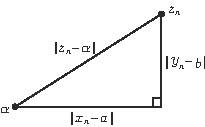
\includegraphics{./Fig/Fig03-A}}
複素数を項とする無限数列 $z_{1}, z_{2}, \ldots, z_{n}, \ldots$ を\textbf{複素数列}とい
う.これを $\{z_{n}\}$ で表す.数列 $\{z_{n}\}$において,$n$ を十分に大きくするとき,$z_n$
が1つの定まった複素数 $\alpha$ に限りなく近づくとき,数列 $\{z_{n}\}$ は$\alpha$に\textbf{収束する}と
いい,これを$\displaystyle \lim_{n\to\infty} z_{n}=\alpha$ あるいは $ z_{n}\to\alpha\, (n\rightarrow\infty)$ のように表す.$z_n$が
$\alpha$に限りなく近づくというのは,点$z_{n}$と$\alpha$の距離
$|z_{n}-\alpha|$ が限りなく0に近づくことである.すなわ
ち $\displaystyle \lim_{n\to \infty}|z_{n}-\alpha|=0$である.$z_{n}=x_{n}+y_{n}i,\, \alpha=a+bi$
とするときは
\[
\begin{array}{lcl}
\dis\lim_{n\rightarrow\infty}z_{n}=\alpha & \Longleftrightarrow &\dis\lim_{n\rightarrow\infty}(x_{n}+y_{n}i)=a+bi\\
&\Longleftrightarrow&\dis \lim_{n\rightarrow\infty}x_{n}=a,\ \lim_{n\rightarrow\infty}y_{n}=b
\end{array}
\]
である.また,数列 $\{z_{n}\}$ が収束しないとき,$\{z_n\}$は\textbf{発散する}という.
\end{Mw}

特に,発散する数列 $\{z_n\}$ について $\displaystyle \lim_{n\rightarrow\infty}|z_{n}|=\infty$ であるとき,$\{z_n\}$は $\infty$ \textbf{に発
散する}といい,$\displaystyle \lim_{n\to\infty} z_{n}=\infty$ あるいは $ z_{n}\rightarrow\infty\, (n\rightarrow\infty)$ と表す.

\noindent
\textbf{[2]\ 無限級数}\par
複素数を項とする無限数列 $\{z_{n}\}$ についても実数列と同様に,「部分和」「無限級数」「無限級数の収束・発散」の意味を定める.
無限級数$\displaystyle \sum^{\infty}_{n=1}z_n$ において,$z_{n}=x_{n}+y_{n}i$ とすると,次が成り立つ.
\[
\sum_{n=1}^{\infty} z_{n}=a+bi\ \Longleftrightarrow\ \sum_{n=1}^{\infty} x_{n}=a,\, \sum_{n=1}^{\infty}y_{n}=b
\]
\step{基本問題を解いてみよう}
\begin{例題}
(1)\ $r >1$ のとき,$\sum_{k=0}^{\infty}\bigg(\displaystyle \frac {\cos x + i \sin x}{r} \bigg)^k
 %%(k= 0,1,2, \ldots)
 $
を求めよ.\par\noindent
(2)\ $\displaystyle r > 1$のとき $\dis \sum_{k=0}^{\infty}\frac{\cos kx}{r^k}$
を求めよ.
\end{例題}

\begin{解答}
(1)  $\dis z = \frac{\cos x + i \sin x}{r}$
とおくと,数列$\{z^k\}\,(k= 0,1,2, \ldots)$の第$n$項までの和$S_n$は
\[
 S_n = 1 + z + z^2 + \cdots + z^{n-1}\quad (n \geqq 1)
\]
$r > 1$であるから$\dis |z| \mathop{=}^{\text{\ajMaruKata{1}}}\footnotetext[1]{$|z|=
\frac{|\cos x+i\,\sin x|}{|r|}=\frac{1}{r}$}
\dfrac{1}{r}<1$\\
したがって\quad$S_n = \frac{1 - z^n}{1 - z}$
\[
\lim_{n \to \infty}\left|S_n - \frac{1}{1-z}\right| \mathop{=}^{\text{\ajMaruKata{2}}} \lim_{n \to \infty}\frac{|z|^n}{|1-z|} = 0
\]よって\footnotetext[2]{$\left|S_n\!-\!\frac{1}{1-z}\right|=
\left|\frac{-z^n}{1-z}\right|=\frac{|z^n|}{|1-z|}=
\frac{|z|^n}{|1-z|}$}
\begin{align*}
\sum_{k=0}^{\infty}z^k &= \lim_{n \to \infty}S_n = \frac{1}{1-z}
=\frac{r}{(r - \cos x) - i \sin x}\\[3mm]
&=\frac{r\{ (r - \cos x) + i \sin x \} }{\{(r - \cos x) - i \sin x\}\{ (r - \cos x) + i \sin x \}}\\[3mm]
&\mathop{=}^{\text{\ajMaruKata{3}}}\frac{r (r - \cos x) + i r \sin x}{r^2 - 2 r \cos x + 1}
\end{align*}\footnotetext[3]{(1行上の分母)$=(r-\cos x)^2+\sin^2x$}
すなわち,求める和は
\[
\sum_{k=0}^{\infty}z^k = \frac{r (r - \cos x)}{r^2 - 2 r \cos x + 1} +i \frac{r \sin x}{r^2 - 2 r \cos x + 1}\tag*{\kotae}
\]

(2)\quad $\begin{array}[t]{lcl}
\dis \sum_{k=0}^{\infty}z^k &=&\dis  \lim_{n \to \infty}\sum_{k=0}^{n}z^k 
\mathop{=}^{\text{\ajMaruKata{4}}} \lim_{n \to \infty}\left( \sum_{k=0}^{n}\frac{\cos kx}{r^k} + i \sum_{k=0}^{n}\frac{\sin kx}{r^k} \right)
\end{array}$\\
であるから,(1)の結果から\footnotetext[4]{ド・モアブルの定理$(\cos x+i\sin x)^k=\cos kx+i\sin kx$}
\[
\sum_{k=0}^{\infty}\frac{\cos kx}{r^k} = \frac{r (r - \cos x)}{r^2 - 2 r \cos x + 1} \tag*{\kotae}
\]

\end{解答}

\section{関数の不定形の極限}
\step{基本を確認しておこう}
一般に,$\lim_{x\to a} f(x)=b,\, \lim_{x\rightarrow a}g(x)=c$であるとき

\begin{Description}{2.5zw}
\item[\hskip1zw a.]
$\lim_{x\rightarrow a} kf (x)=kb$\quad($k$は定数)
\item[\hskip1zw b.]
$\lim_{x\rightarrow a}\{f(x)\pm g(x)\}=b\pm c$\quad(複号同順)
\item[\hskip1zw c.]
$\lim_{x\rightarrow a}f(x)g(x)=bc$
\item[\hskip1zw d.]
$\lim_{x\to a}\dfrac{f(x)}{g(x)}=\dfrac{b}{c}$\quad(ただし,$g(x)\neq 0,\, c\neq 0)$
\end{Description}
が成り立つ.$x\rightarrow a$ の代わりに $x\rightarrow\infty$,$x\rightarrow-\infty$ としても同様に成立する.

しかし,$\lim_{x\to -3}\dfrac{x^{3}+27}{x^{2}-9}, \lim_{x\rightarrow\infty}\dfrac{5x^{2}+4x}{3x^{2}-x+2}, \lim_{x\rightarrow\infty} (\sqrt{x+3}-\sqrt{x})$ などは,形式的には,
$\dfrac{0}{0}$,$\dfrac{\infty}{\infty}$,$\infty-\infty$と表せるが,このままでは実際の極限値は不明である.このよう
な形を\textbf{不定形}と呼ぶが,いろいろな工夫を施して不定形ではないようにする必要
がある.不定形の極限は,上記のほかに $0\times\infty$,$\infty^{0}$,$1^{\infty}$,$0^{0}$ などの形があるが,代表
的なものの処理のコツを次に示す.
\begin{shadebox}
\begin{Description}{8.5zw}
\item[a.\quad $\dfrac{0}{0}$の形]有理式の場合,約分する\\
無理式の場合,分母または分子を有理化する
\item[b.\quad $\dfrac{\infty}{\infty}$の形] 分数式の場合,分母の最高次の項で分母・分子を割る
\item
[c.\quad $\infty-\infty$の形]整式の場合,最高次の項でくくり出す\\
無理式の場合,有理化する\\
$\left(\sqrt{A}-\sqrt{B}=\dfrac{A-B}{\sqrt{A}+\sqrt{B}}\right)$
\end{Description}
\end{shadebox}
\step{基本問題を解いてみよう}
\begin{例題}
次の極限をそれぞれ求めよ.
\begin{longtable}[l]{@{}l@{\hskip1zw}l}
(1)\quad  $\lim_{x\rightarrow 2}\dfrac{\sqrt{x+2}-\sqrt{3x-2}}{\sqrt{4x+1}-\sqrt{5x-1}}$ & (2)\quad $\lim_{x\to -\infty}\dfrac{x^4+3x-8}{2x^3-5x^2+7}$
\\[2mm]
(3)\quad $\lim_{x\rightarrow\infty}(\sqrt{x^{2}-x+1}-\sqrt{x^{2}+3x-1})$&  (4)\quad $\lim_{x\rightarrow\infty}(x-\sqrt{2x+1})$
\end{longtable}
\end{例題}

\begin{解答}\vspace{-\baselineskip}\vspace{-.55\baselineskip}
\begin{fleqn}[4zw]
\begin{alignat}{1}
(1)\ &\phantom{=}\;\lim_{x\to2}\dfrac{\sqrt{x+2}-\sqrt{3x-2}}{\sqrt{4x+1}-\sqrt{5x-1}}\notag\\[3mm]
&=\Mframe{\lim_{x\to2}\dfrac{(x+2-3x+2) (\sqrt{4x+1}+\sqrt{5x-1})}{(4x+1-5x+1)
(\sqrt{x+2}+\sqrt{3x-2})}}\Footnotemark[1]\notag\\[3mm]
&=\lim_{x\to 2}\dfrac{-2(x-2)(\sqrt{4x+1}+\sqrt{5x-1})}{-(x-2)(\sqrt{x+2}+\sqrt{3x-2})}\notag\\[3mm]
&=\lim_{x\rightarrow 2}\dfrac{2(\sqrt{4x+1}+\sqrt{5x-1})}{\sqrt{x+2}+\sqrt{3x-2}}=\dfrac{2(3+3)}{2+2}=3\tag*{\hbox to1zw{\hss\Kotae}}
\end{alignat}\footnotetext[1]{分母・分子がともに無理式で,$\frac{0}{0}$の不定形の場合,分母・分子の両方を有理化する.}
\end{fleqn}

\noindent
(2)\quad$\Mframe{x=-t}\Footnote[2]{$\lim_{x\to-\infty}f(x)$は$x=-t$とおいて,
$\lim_{t\to\infty}g(t)$の形に帰着させる.}$とおくと,$x\to-\infty$のとき$t\to\infty$.
\begin{align*}
&\lim_{x\rightarrow-\infty}\dfrac{x^{4}+3x-8}{2x^{3}-5x^{2}+7}\\
=\;&\Mframe{\lim_{t\rightarrow\infty}\dfrac{t^{4}-3t-8}{-2t^{3}-5t^{2}+7}}\Footnotemark[3]
=\lim_{t\rightarrow\infty}\dfrac{t-\dfrac{3}{t^{2}}-\dfrac{8}{t^{3}}}{-2-\dfrac{5}{t}+\dfrac{7}{t^{3}}}=-\infty\tag*{\Kotae}
\end{align*}%
\footnotetext[3]{$\frac{\infty}{\infty}$の不定形
である.分母の最高次の項で分母・分子を割る.}\footnotetext[4]{無理式で$\infty-\infty$の不定形である.与式
$=\frac{\sqrt{\quad}\;\text{\raisebox{-.5mm}{$-$}}\;\sqrt{\quad}}{1}$と考えて,分子を有理化する.}
\begin{fleqn}
\begin{alignat*}{2}
(3)\quad&\dis\Mframe{\lim_{x\to\infty}(\sqrt{x^{2}-x+1}-\sqrt{x^{2}+3x-1})}\Footnotemark[4]\\[3mm]
&\dis=\lim_{x\rightarrow\infty}\dfrac{(x^{2}-x+1)-(x^{2}+3x-1)}{\sqrt{x^{2}-x+1}+\sqrt{x^{2}+3x-1}}\\[3mm]
&\dis=\lim_{x\rightarrow\infty}\dfrac{-4x+2}{\sqrt{x^{2}-x+1}+\sqrt{x^{2}+3x-1}}\\[3mm]
&\dis\mathop{=}^{\text{\ajMaruKata{5}}}\lim_{x\rightarrow\infty}\dfrac{-4+\dfrac{2}{x}}{\sqrt{1-\dfrac{1}{x}+\dfrac{1}{x^{2}}}+\sqrt{1+\dfrac{3}{x}-\dfrac{1}{x^{2}}}}
=\dfrac{-4}{2}=-2\tag*{\Kotae}
\end{alignat*}
\footnotetext[5]{分母・分子を$\sqrt{x^2}=x$で割った.}

\footnotetext[6]{$\infty-\infty$の不定形で無理式だから有理化をしそうであるが,$x$と$\sqrt{2x+1}$では$x$のほうが高次だから$x$でくくった.}
\begin{alignat*}{2}
(4)\quad&\lim_{x\rightarrow\infty}(x-\sqrt{2x+1})\\
&\mathop{=}^{\text{\ajMaruKata{6}}} \lim_{x\rightarrow\infty}x\left(1-\dfrac{\sqrt{2x+1}}{x}\right)
=\lim_{x\rightarrow\infty}x\left(1-\sqrt{\dfrac{2}{x}+\dfrac{1}{x^2}}\right)
\mathop{=}^{\text{\ajMaruKata{7}}}\infty\tag*{\Kotae}
\end{alignat*}\footnotetext[7]{$\infty\times1$より極限は$\infty$.}
\end{fleqn}
\end{解答}


\section{重要な極限(1)}
\step{基本を確認しておこう}

三角関数についての$ \frac{0}{0}$ の不定形である.

三角関数の不定形の極限では,次の2つの公式に帰着させて考えるのが原則である.

\begin{shadebox}
\begin{center}
\mbox{$\lim_{\Textcircled{$\theta$} \rightarrow 0}\frac{\sin \Textcircled{$\theta$}}{\Textcircled{$\theta$}} =1,\quad \lim_{\theta \rightarrow 0}\frac{\tan\theta}{\theta}=1 \quad \mbox{\small(ただし,$\theta$は弧度法で表されている)}$}
\end{center}
\end{shadebox}

たとえば,$ab\neq 0$ のとき $\lim_{\theta \rightarrow 0}\frac{\sin a\theta}{b\theta}=\lim_{\theta\rightarrow 0}\frac{\sin a\theta}{a\theta}\cdot\frac{a}{b}=1\cdot\frac{a}{b}=\frac{a}{b}$
\begin{align*}
\lim_{\theta\rightarrow 0}\frac{1-\cos\theta}{\theta^{2}}&=\lim_{\theta\rightarrow 0}\frac{(1-\cos\theta)(1+\cos\theta)}{\theta^{2}(1+\cos\theta)}=\lim_{\theta\rightarrow 0}\frac{\sin^{2}\theta}{\theta^{2}(1+\cos\theta)}\\
&=\lim_{\theta\rightarrow 0}\left(\frac{\sin\theta}{\theta}\right)^{2}\cdot\frac{1}{1+\cos\theta}=1^{2}\cdot\frac{1}{2}=\frac{1}{2}
\end{align*}
となる.この2つの結果は公式として覚えておくとよい.

さらに,$a\neq 0$ のとき
\[
\lim_{x \rightarrow \infty}x\sin\frac{a}{x}=\lim_{t \rightarrow 0}\frac{\sin at}{t}=a \quad \left(x=\frac{1}{t} とおいた \right)
\]
となる.ただし,$\lim_{x\rightarrow 0}x\sin\frac{1}{x}$ は $\left |\sin\frac{1}{x}\right |\leqq 1$ から $0\leqq \left |x\sin\frac{1}{x}\right |\leqq |x|$ となり,はさみうちの原理から与式 $=0$ となる.

\step{基本問題を解いてみよう}
\begin{例題}
次の極限を求めよ.\par
\begin{longtable}[l]{@{}l@{\hskip4zw}l}
(1)\quad$\lim_{x\rightarrow 0}\frac{\cos 7x-\cos 3x}{x^{2}}$ & (2)\quad$\lim_{x\rightarrow 0}\frac{\tan^{3}x-\sin^{3}x}{x^{5}}$\\[3mm]
(3)\quad$\lim_{x\rightarrow \frac{\pi}{2}}\frac{1-\cos(1-\sin x)}{\cos^{4}x}$&
\end{longtable}
\end{例題}

\begin{解答}
\begin{fleqn}[4zw]
$\begin{array}[t]{ll}
(1)\quad\cos 7x-\cos 3x\, &\mathop{=}^{\text{\ajMaruKata{1}}}-2\sin\frac{7x+3x}{2}\sin\frac{7x-3x}{2}\\[3mm]
&=-2\sin 5x\sin 2x \quad から
\end{array}$\footnotetext[1]{和積の公式
$\cos A-\cos B=-2\sin\frac{A+B}{2}\sin\frac{A-B}{2}$より.
}\par
\begin{alignat}{2}
&与式\, &=&\lim_{x\rightarrow 0}\frac{-2\sin 5x\sin 2x}{x^{2}}=\lim_{x\rightarrow 0}(-2)\cdot\frac{\sin 5x}{5x}\cdot \frac{\sin 2x}{2x}\cdot 10\notag\\[3mm]
&&=&\;(-2)\cdot 1\cdot 1\cdot 10=-20\tag*{\kotae}
\end{alignat}
\end{fleqn}
\begin{fleqn}[1.5zw]
$(2)\quad\lim_{x\rightarrow 0}\frac{\tan^{3}x-\sin^{3}x}{x^{5}}=\lim_{x\rightarrow 0}\frac{\sin^{3}x(1-\cos^{3}x)}{x^{5}\cos^{3}x}$\\
\begin{alignat}{2}
&&=&\lim_{x \rightarrow 0}\frac{\sin^3 x(1-\cos x)(1+\cos x+\cos^{2}x)}{x^{5}\cos^{3}x}\notag\\[3mm]
&&\mathop{=}^{\text{\ajMaruKata{2}}}&\lim_{x \rightarrow 0}\frac{\sin^3x\sin^2x(1+\cos x+\cos^{2}x)}{x^{5}(1+\cos x)\cos^{3}x}\notag\\[3mm]
&&=&\lim_{x\rightarrow 0}\left (\frac{\sin x}{x}\right )^{5}\cdot\frac{1+\cos x+\cos^{2}x}{(1+\cos x)\cos^{3}x}=1\cdot\frac{3}{2\cdot 1}=\frac{3}{2}\tag*{\Kotae}
\end{alignat}\footnotetext[2]{分母・分子に$1+\cos x$を掛けた.あるいは
$1-\cos x=2\sin^2\frac{x}{2}$を用いてもよい.}
$(3)\quad\frac{\pi}{2}-x=t とおくと \cos x=\cos\left (\frac{\pi}{2}-t\right )=\sin t\\
\quad1-\sin x=1-\sin\left (\frac{\pi}{2}-t\right )=1-\cos t\mathop{=}^{\text{\ajMaruKata{3}}}2\sin^{2}\frac{t}{2}$\footnotetext[3]{半角の公式より.}\footnotetext[4]{%
	分子に再び半角の公式を用いた.
	}\footnotetext[5]{$t\to0$のとき$\sin^2\frac{t}{2}\to0$より,
	$\sin^2\frac{t}{2}=\theta$とすると
	$\lim_{t\to0}\frac{\sin\left(\sin^2\frac{t}{2}\right)}{\sin^2\frac{t}{2}}
	=\lim_{\theta\to0}\frac{\sin\theta}{\theta}=1
	$となる.}
\begin{alignat}{2}
&与式\, &=&
\lim_{t\rightarrow 0}\frac{1-\cos\left (2\sin^{2}\frac{t}{2}\right )}{\sin^{4}t}\notag\mathop{=}^{\text{\ajMaruKata{4}}}\lim_{t\rightarrow 0}\frac{2\sin^{2}\left (\sin^{2}\frac{t}{2}\right )}{\sin^{4}t}\notag\\[3mm]
&&=&\lim_{t\rightarrow 0}2\left (\frac{t}{\sin t}\right )^{4}\cdot
\Mframe{\left\{\frac{\sin\left (\sin^{2}\frac{t}{2}\right )}{\sin^{2}\frac{t}{2}}\right\}^{2}}\Footnotemark[5]\cdot\left (\frac{\sin\frac{t}{2}}{\frac{t}{2}}\right )^{4}\cdot\frac{1}{2^{4}}\notag\\[3mm]
&&=&\;2\cdot 1\cdot 1\cdot 1\cdot\frac{1}{2^{4}}=\frac{1}{8}\tag*{\kotae}
\end{alignat}
\end{fleqn}
\end{解答}

\section{重要な極限(2)}
\step{基本を確認しておこう}

次の定義はきわめて重要である.

\begin{shadebox}
\begin{center}
$\lim_{\text{\Textcircled{$h$}} \rightarrow 0}(1+\Textcircled{$h$})
^{\frac{1}{\text{\Textcircled{$h$}}}} = e \quad (e=2.71828 \cdots)$
\end{center}
\end{shadebox}

\VS{-.5}
$e$は\textbf{自然対数の底}と呼ばれる無理数である.これより次の公式が導かれる.

\begin{titlebox}{指数関数・対数関数に関する極限}
\begin{fleqn}
\begin{align*}
(1)\ &\lim_{x \rightarrow \pm \infty}\left(1+\frac{1}{x}\right)^x = e\hskip4zw
(2)\ \lim_{x \rightarrow 0}\frac{e^x - 1}{x} = 1\\
(3)\ &\lim_{x \rightarrow 0}\frac{a^x - b^x}{x} = \log_e\frac{a}{b} \enskip(a>0,\,b>0)
\end{align*}
\end{fleqn}
\end{titlebox}
\begin{証明}(1)\ 
$x = \frac{1}{h}$ とおくと,$
\lim_{x\rightarrow\pm\infty}\left(1+\frac{1}{x}\right)^{x}=\lim_{h\rightarrow\pm 0}(1+h)^{\frac{1}{h}}=e$
\\
(2)\ $e^{x}-1=h$ とおくと $x=\log_{e}(1+h)$ で $h\rightarrow 0$ だから
\[
\lim_{x\rightarrow 0}\frac{e^{x}-1}{x}=\lim_{h\rightarrow 0}\frac{h}{\log_{e}(1+h)}=\lim_{h\rightarrow 0}\frac{1}{\log_{e}(1+h)^{\frac{1}{h}}}=\frac{1}{\log_{e}e}=1
\]
(3)\ $a>0,\, b>0$ のとき
\begin{align*}
\lim_{x\rightarrow 0}\frac{a^{x}-b^{x}}{x}&=\lim_{x\rightarrow 0}\frac{b^{x}\{(\frac{a}{b})^{x}-1\}}{x}=\lim_{x\rightarrow 0}b^{x}\cdot\lim_{x\to0}\frac{(\frac{a}{b})^{x}-1}{x}\\
&=1\cdot\log_{e}\frac{a}{b}=\log_{e}\frac{a}{b}
\end{align*}
\begin{shadebox}
$a>1$のとき,$\lim_{x\to \infty}\frac{x}{a^x}=0$
\end{shadebox}
\end{証明}

\begin{証明}
$x\to\infty$より,十分大きな自然数$n$に対して$n\le x<n+1$として考えると,$a^x\ge a^n\,(>0)$だから
\[
0<\frac{x}{a^x}<\frac{n+1}{a^n}
\]
$a>1$のとき$a=1+h\,(h>0)$とおけるから,2項定理により$n\ge2$のとき
\begin{align*}
a^n & = (1+h)^n= {}_n\mathrm{C}_0+{}_n\mathrm{C}_1\,h+{}_n\mathrm{C}_2\,h^2+\cdots+{}_n\mathrm{C}_n\,h^n\\
&>{}_n\mathrm{C}_2\,h^2=\frac{n(n-1)}{2}h^2\,(>0)
\intertext{ゆえに}
&\frac{n+1}{a^n}<\frac{n+1}{\frac{n(n-1)}{2}h^2}=
\frac{2(n+1)}{n(n-1)h^2}=\frac{2(1+\frac{1}{n})}{(n-1)h^2}
\end{align*}
ここに,$x\to \infty$のとき$n\to\infty$であるから,
\[
0\le\lim_{x\to\infty}\frac{x}{a^x}\le\lim_{n\to\infty}\frac{n+1}{a^n}
\le\lim_{n\to \infty}\frac{(1+\frac{1}{n})}{(n-1)h^2}=0
\]
よって,はさみうちの原理から
\[
a>1のとき\quad \lim_{x\to\infty}\frac{x}{a^x}=0\tag*{(証明終)}
\]
\end{証明}
\step{基本問題を解いてみよう}
\begin{例題}
次の極限を求めよ.

\begin{fleqn}
\begin{alignat*}{2}
(1)\quad & \lim_{x\rightarrow 0}\frac{\log_{2}(a+3x)-\log_{2}a}{x}\quad && (a>0)\\
(2)\quad& \lim_{x\rightarrow 0}\frac{e^{\sin 3x}-e^{-2x}}{x} && (3)\enskip\lim_{x\rightarrow\infty}\left(1+\frac{1}{x}+\frac{1}{x^2}\right)^2
\end{alignat*}
\end{fleqn}
\end{例題}

\enlargethispage{3mm}
\begin{解答}\vspace{-1.5\baselineskip}
\begin{align*}
(1)\enskip&\lim_{x \rightarrow 0}\frac{\log_2(a + 3x) - \log_2a}{x}\\
&=\lim_{x \rightarrow 0}\frac{\log_2\left(1 + \frac{3x}{a}\right)}{x} 
\mathop{=}^{\text{\ajMaruKata{1}}} \lim_{x \rightarrow 0}\frac{\log_2\left(1 + \frac{3x}{a}\right)}{\frac{3x}{a}} \cdot \frac{3}{a}\\
&=\lim_{x \rightarrow 0}\frac{3}{a}\log_2\left(1 + \frac{3x}{a}\right)
^{\frac{1}{\frac{3x}{a}}} = \frac{3}{a}\log_2e\tag*{\kotae}
\end{align*}\footnotetext[1]{%
	$\lim_{f(x)\to0}\{1+f(x)\}^{\frac{1}{f(x)}}=e$を用いるために,
	分母を$\frac{3x}{a}$に直した.
	}
\begin{fleqn}
\begin{align*}
(2)\enskip&\lim_{x \rightarrow 0}\frac{e^{\sin3x}-e^{-2x}}{x}\mathop{=}^{\text{\ajMaruKata{2}}}\lim_{x \rightarrow 0}\frac{e^{\sin3x}-1-(e^{-2x}-1)}{x}\\
&=\lim_{x \rightarrow 0}\left(\frac{e^{\sin3x}-1}{\sin3x}\cdot \frac{\sin3x}{3x}\cdot 3 + \frac{e^{-2x}-1}{-2x}\cdot2\right)\\
&=1\cdot 1\cdot 3+1\cdot 2=5\tag*{\kotae}
\end{align*}\footnotetext[2]{%
	$\lim_{f(x)\to0}\frac{e^{f(x)}-1}{f(x)}=1$を用いるために,分子を変形した.
	}%
\end{fleqn}%
%(3)\quad \Mframe{xは十分大きい正の数と考えてよい}\Footnote[3]{%
%	$x\to\infty$より.
%	}ので,自然数 $n$ に対して $n\leqq x<n+1$ とすると
%\[
%\Mframe{\dis
%0<\frac{x}{3^{x}}<\frac{n+1}{3^{n}}}
%\Footnotemark[4]\tag*{$\cdots\cdots$ ①}
%\]
%
%ここで,\Mframe{2項定理}\footnotetext[4]{$y=3^x$のグラフは単調増加だから,$n<2^n\leq3^x<3^{n+1}$より
%$\frac{1}{3^{n+1}}<\frac{1}{3^x}\leq\frac{1}{3^n}$
%したがって$0<\frac{n}{3^{n+1}}<\frac{x}{3^x}<\frac{n+1}{3^n}$
%}\Footnote[5]{%
%	$(a+b)^n={}_n\mathrm{C}_0a^n+{}_n\mathrm{C}_1a^{n-1}b
%	+\cdots+{}_n\mathrm{C}_r a^{n-r}b^r
%	+\cdots+{}_n\mathrm{C}_nb^n
%	$
%	}により $n\geqq 2$ のとき
%\begin{align}
%3^{n}&=(1+2)^{n}={}_n\mathrm{C}_0 + {}_n\mathrm{C}_1 \cdot 2+{}_n\mathrm{C}_2 \cdot 2^2 + \cdots + {}_n\mathrm{C}_n2^n\notag\\
%&>{}_n\mathrm{C}_2\cdot 2^2=\frac{n(n-1)}{2}\cdot 2^{2}=2n(n-1)\tag*{$\cdots\cdots$②}
%\end{align}
%
%①, ②から\par
%\[
%0<\frac{x}{3^{x}}<\frac{n+1}{2n(n{-1)}}=\frac{1+\frac{1}{n}}{2(n-1)}
%\]
%ここに,$ x\rightarrow\infty$ のとき $ n\rightarrow\infty$ だから\par
%\[
%0\leqq \lim_{x \rightarrow \infty}\frac{x}{3^{x}}\leqq \lim_{x \rightarrow \infty}\frac{1+\frac{1}{n}}{2(n{-1)}}=0
%\]
%
%よって,はさみうちの原理から
%\[
%\lim_{x \rightarrow \infty}\frac{x}{3^{x}}=0 \tag*{\kotae}
%\] 
\end{解答}%%
(3)$\displaystyle \lim_{x \to \infty} \left( 1+\frac{1}{x}+\frac{1}{x^2} \right)^x$ において,
$x=\dfrac{1}{y}$とおくと$x \to \infty$のとき$y \to 0$\\
したがって,
\[
 \lim_{x \to \infty} \left( 1+\dfrac{1}{x}+\dfrac{1}{x^2} \right)^x
=\lim_{y \to 0} (1+y+y^2)^{\frac{1}{y}}
\]
さらに
$\Mframe{y+y^2=z\text{とおく}}\Footnote[3]{$y \to 0$のとき$y+y^2 \to 0 $であるから,
$\displaystyle \lim_{z \to 0} (1+z)^\frac{1}{z} =1$を用いることができるのではないかと予想して$y+y^2=z $とおいた.}$
と,$y \to 0$のとき$z \to 0$であり
\[
 \lim_{y \to 0} (1+y+y^2)^{\frac{1}{y}}
=\lim_{\begin{subarray}{c}
	y \to 0\\ z \to 0
	\end{subarray}
	}    (1+z)^{\frac{1}{y}}
=\lim_{
	\begin{subarray}{c}
	y \to 0\\
	z \to 0
	\end{subarray}
	} \{ (1+z)^{\frac{1}{z}} \}^{\frac{z}{y}}
\]
ここで,
$\displaystyle 
 \lim_{y \to 0} \frac{z}{y}  
=\lim_{y \to 0} \frac{y+y^2}{y} =\lim_{y \to 0} (1+y) =1$

よって,$\text{与式}=e^1=e  $\kotae
\pagebreak[3]

\section{微分係数の定義}
\step{基本を確認しておこう}

\begin{Mw}{45mm}{\hfill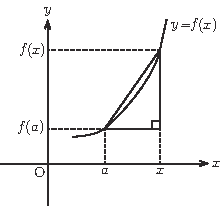
\includegraphics{./Fig/Fig03-B}}
連続関数 \mbox{$y=f(x)$}の定義域内の2点 $a,\linebreak x$ に対して $\lim_{x\rightarrow a}\frac{f(x)-f(a)}{x-a}$,すなわち,$\lim_{h\rightarrow 0}\frac{f(a+h)-f(a)}{h}$ が存在して有限確定ならば,$x=a$ において\textbf{微分可能}といい,この極限値を関数 $f(x)$ の $x=a$ における\textbf{微分係数}あるいは,\textbf{微係数}といい,$f'(a)$ と表す.また,
\begin{align*}
&\lim_{x\rightarrow a+0}\frac{f(x)-f(a)}{x-a}\quad すなわち \quad \lim_{h\rightarrow+0}\frac{f(a+h)-f(a)}{h}\\
&\lim_{x\rightarrow a-0}\frac{f(x)-f(a)}{x-a}\quad すなわち \quad \lim_{h\rightarrow-0}\frac{f(a+h)-f(a)}{h}
\end{align*}
が存在して有限確定ならば,それぞれ $x=a$ において\textbf{右側微分可能},\textbf{左側微分可能}といい,これらの極限値を $f_{+}'(a)$,$f_{-}'(a)$ と表し,関数 $f(x)$ の $x=a$ における\textbf{右側微分係数},\textbf{左側微分係数}という.
\end{Mw}

\begin{shadebox}
\centering
$f(x)$が$x=a$で微分可能\quad$\Longleftrightarrow$\quad$f_{+}'(a)=f_{-}'(a)$
\end{shadebox}
\pagebreak[3]

\VS{-.5}
さて,微分可能な関数 $f(x)$ は連続である.

\begin{証明}$f(x)$ が $x=a$ で微分可能であるならば,
\[
\lim_{x\rightarrow a}\{f(x)-f(a)\}=\lim_{x\rightarrow a}\frac{f(x)-f(a)}{x-a}\cdot(x-a)=f'(a)\cdot 0=0
\]
よって,$\lim_{x\rightarrow a}f(x)=f(a)$ となり,$f(x)$ は $x=a$ で連続である.\hfill(証明終)
\end{証明}

\step{基本問題を解いてみよう}
\begin{例題}
次の関数の与えられた点における微分係数を定義により求めよ.\par
\begin{longtable}[l]{@{}ll}
(1)\quad$f(x)=\frac{1}{x}\quad (x=a\neq 0)$ &(2)\quad$f(x)=\sqrt[3]{x}\quad (x=a)$ \\[3mm]
(3)\quad$f(x)=\left\{\begin{array}{ll}
x\sin\frac{1}{x} & (x\neq 0)\\
0 & (x=0)
\end{array}\right.$
\quad$(x=0)$
\end{longtable}
\end{例題}

\begin{解答}$(1)\quad f'(a) = \lim_{h \rightarrow 0}\frac{f(a+h)-f(a)}{h}$
\[
=\lim_{h \rightarrow 0}\frac{1}{h}\left (\frac{1}{a+h} - \frac{1}{a} \right) =\lim_{h \rightarrow 0}\frac{-1}{(a+h)a}=-\frac{1}{a^2}\tag*{\kotae}
\]
\begin{別解}
$f'(a)=\lim_{x\to a}\frac{f(x)-f(a)}{x-a}=\lim_{x\to a}
\frac{\frac{1}{x}-\frac{1}{a}}{x-a}$
\end{別解}
\begin{fleqn}[1.5zw]
(2)\hspace{1zw}(i)\quad $a \neq 0$のとき
\begin{alignat}{2}
&f'(a) &=&\lim_{x\rightarrow a}\frac{f(x) - f(a)}{x-a}=\lim_{x\rightarrow a}\frac{\sqrt[3]{x} - \sqrt[3]{a}}{x-a}\notag\\[3mm]
&&=&\lim_{x\rightarrow a}\frac{\sqrt[3]{x} - \sqrt[3]{a}}{(\sqrt[3]{x} - \sqrt[3]{a})(\sqrt[3]{x^2} + \sqrt[3]{x}\sqrt[3]{a} + \sqrt[3]{a^2})}\notag\\[3mm]
&&=&\lim_{x\rightarrow a}\frac{1}{\sqrt[3]{x^2} + \sqrt[3]{x}\sqrt[3]{a} + \sqrt[3]{a^2}} \mathop{=}^{\text{\ajMaruKata{1}}}\frac{1}{3\sqrt[3]{a^2}}\tag*{\kotae}
\end{alignat}\footnotetext[1]{最初から$a\not=0$と$a=0$の場合分けには気づかないかもしれないが,\ajMaruKata{1}の所で場合分けに気づくことになる.}%
(ii)\quad$a = 0$のとき
\[
f'(0) =\lim_{x\rightarrow 0}\frac{f(x) - f(0)}{x}=\lim_{x\rightarrow0}\frac{\sqrt[3]{x}}{x} = \lim_{x\rightarrow 0}\frac{1}{\sqrt[3]{x^2}}
=\infty\tag*{\kotae}
\]
(3)\hspace{1zw}$\lim_{x\rightarrow 0}\frac{f(x) - f(0)}{x}=\lim_{x\rightarrow 0}\frac{x \sin \frac{1}{x}}{x}=\lim_{x\rightarrow 0}\sin \frac{1}{x}$
%
%\Mframe{\sin\frac{1}{x}はx \rightarrow 0のとき有限確定値あるいは\infty,-\infty のいずれにもならない}\,\Footnote[2]{%
%	$x=\frac{1}{\pi},\frac{1}{2\pi},\ldots,\frac{1}{n\pi},\ldots$の値をとりながら,$x\to0$のとき$\lim_{x\to0}\sin\frac{1}{x}=0x=\frac{2}{\pi},\frac{2}{5\pi},\ldots,\frac{2}{(4n+1)\pi},\ldots$の値をとりながら,$x\to0$のとき$\lim_{x\to0}\sin\frac{1}{x}=1$両者が一致しないので,極限は存在しない.
%	}\linebreak
%	ので,$f'(0)$は存在しない.\kotae

$x>0$において,$\sin \dfrac{1}{x}=0$となるのは
$\dfrac{1}{x}=n\pi$より$x=\dfrac{1}{n\pi}\, (n=1,2,\ldots)$のときである.

また,$\sin \dfrac{1}{x}=1$となるのは
$\dfrac{1}{x}=\dfrac{\pi}{2}+2(n-1)\pi=\dfrac{4n-3}{2}\pi$より
$x=\dfrac{1}{(4n-3)\pi}\, (n=1,2,\ldots)$のときである.

したがって,$x=\dfrac{1}{\pi},\, \dfrac{1}{2\pi},\, \ldots , \, \dfrac{1}{n\pi}, \ldots$の値をとりながら
$x$が限りなく0に近づくとき,$\sin \dfrac{1}{x}$の値はつねに0となる.

また,$x=\dfrac{2}{\pi}, \, \dfrac{2}{5\pi}, \, \ldots , \,  \dfrac{1}{(4n-3)\pi}, \, \ldots$の値をとりながら
$x$が限りなく0に近づくとき,$\sin \dfrac{1}{x}$の値はつねに1となる.

これらの結果から$\displaystyle \lim_{x \to 0} \sin \frac{1}{x}$は存在しない.

よって,$f'(0)$は存在しない.\kotae

\end{fleqn}

\step{過去問題にチャレンジ!}
\medskip
\begin{問題}[1]
正の整数$n$ に対して,$1\times 3\times \cdots \times( 2n-1 )=( 2n-1 )!!$ と表すことにします.
このとき,次の極限値を求めなさい.
\[
\lim_{n\to\infty}\frac{\sqrt[n]{( 2n-1)!!}}{n}
\]
\end{問題}
\begin{解答}
自然対数をとって考える.$(2n-1)!!=\frac{(2n)!}{(2n)!!}$より
\begin{fleqn}
\begin{align*}
&\log_{e}\frac{\sqrt[n]{\left( 2n-1 \right)!!}}{n}=\log_{e}\frac{1}{n}\sqrt[\text{\raisebox{3mm}{\scalebox{1.1}{$n$}}}]{\frac{(2n)!}{(2n)!!}}\\
	=&\;\log_{e}\sqrt[\text{\raisebox{3mm}{$n$}}]{\left(\frac{n}{2}\times \frac{n}{4}\times\cdots\times
\frac{n}{2n} \right)\times \left(\frac{1}{n}\times \frac{2}{n}\times\cdots\times \frac{2n}{n} \right)}\\
	=&\;
\frac{1}{n}\left(\sum\limits_{k=1}^n \log_{e}
\frac{n}{2k}+\sum_{k=1}^{2n} \log_{e}
\frac{k}{n}\right)
=\frac{1}{n}\sum\limits_{k=1}^n \left\{-\log_{e}\left(
2\cdot \frac{k}{n}\right) \right\} +\frac{1}{n}\sum\limits_{k=1}^{2n} \log_{e}\frac{k}{n} 
\end{align*}
\end{fleqn}
 よって
\begin{fleqn}[2zw]
\begin{align*}
&\lim_{n\to\infty}\log_{e}\frac{\sqrt[n]{\left(2n-1\right)!!}}{n}\\
&=\lim_{n\to\infty}\frac{1}{n}\sum\limits_{k=1}^n
\left\{-\log_{e}\left(2\cdot \frac{k}{n} \right) \right\}+\lim_{n\to\infty}
\frac{1}{n}\sum\limits_{k=1}^{2n} \log_{e}\frac{k}{n}\\
&=-\int_{0}^1 \log_{e} 2x\, dx+\int_0^2\log_{e}x\,dx\\
&=-[x\log_e2x-x]_0^1+[x\log_e x-x]_0^2=\log_e\frac{2}{e}
\end{align*}
\end{fleqn}
ゆえに
\[
\lim_{n\to\infty}
\frac{\sqrt[n]{(2n-1)!!}}{n}=\frac{2}{e}\tag*{\Kotae}
\]
\end{解答}
\begin{解説}
\Mframe{区分求積法}\Footnote[1]{第3章9節で学ぶ.}を用いる.なお次も有用である.
\end{解説}
\begin{titlebox}{スターリングの公式}
$n\to \infty$のとき(両辺の比$\to1$という意味で)
\[
n!\sim \sqrt{2\pi n}\left(\frac{n}{e} \right)^{n}\hskip3zw
\text{\null($e$は自然対数の底)}
\]
\end{titlebox}
これを用いると,$n\to \infty $のとき,次のようにも求められる.
\begin{fleqn}
\begin{align*}
\frac{\sqrt[\text{\raisebox{1.5mm}{$n$}}]{\left( 2n-1 \right)!!}}{n}
 &=\frac{1}{n}\sqrt[\text{\raisebox{3mm}{$n$}}]{\frac{(2n)!}{2^{n}\times n!}}\, \sim \, 
\frac{1}{2n}\sqrt[\text{\raisebox{3mm}{$n$}}]{\sqrt {2\pi \times 2n} \left( \frac{2n}{e} 
\right)^{2n}\div \sqrt {2\pi n} \left( \frac{n}{e} \right)^{n}}\\
& =\frac{1}{2n}\sqrt[\text{\raisebox{2.8mm}{$n$}}]{\sqrt{2}\! \times\! 2^{2n}\!\times\! 
\left(\frac{n}{e} \right)^{n}}\!\! =\frac{1}{2n}\times \frac{n}{e}\times 
4\times\!\! \sqrt[2n]{2}= \frac{2}{e}\times\!\! \sqrt[{2n}]{2}\sim \frac{2}{e}
\end{align*}
\end{fleqn}
\begin{問題}[2]
$f(x)$は\Mframe{C^{n}級}\Footnote[2]{第2章で学ぶ.}の関数($f'(x),f''(x),\ldots,f^{(n)}(x):\,n$次までの導関数が連続な関数)とし,しかも$f(0)=f'(0)=\cdots =f^{(n)}(0)=0$と仮定します.

$
\lim_{x\to0}\frac{f^{(n)}(x)\cdot \sin x}{f^{(n-1)}(x)}=1$ 
のとき,$\lim_{x\to0}\frac{f^{(n)}(x)}{f(x)}(\sin x)^{n}$を求めなさい.
\end{問題}


\begin{解答}
\begin{fleqn}[2zw]
\[
\frac{f^{(n)}(x)}{f(x)}(\sin x)^{n}=\frac{f^{(n)}(x)\sin x}{f^{( n-1 )}( x )}\times\frac{f^{( n-1 )}( x )\sin x}{f^{( n-2 )}( x )}\times \cdots \times \frac{f^{(1)}(x)\sin x}{f( x )}
\]
\end{fleqn}
\end{解答}
ロピタルの定理より
\begin{fleqn}[4zw]
\begin{align*}
\lim_{x\to0}\frac{f^{(n-1)}(x)\sin x}{f^{(n-2)}(x)}&=\lim_{x\to0} \frac{\{f^{(n-1)}(x)\cdot \sin x \}'}{\{f^{(n-2)}(x) \}'}\\
	& =\lim_{x\to0} \frac{f^{(n)}(x)\sin x +f^{(n-1)}(x)\cos x}{f^{(n-1)}(x)}\\
	&=1+\lim_{x\to0}\cos x=2\\
\lim_{x\to0}\frac{f^{(n-2)}(x)\sin x}{f^{(n-3)}(x)}
	&=\lim_{x\to0}\frac{\{f^{(n-2)}(x)\sin x \}'}{\{ f^{(n-3)}(x)\}'}\\
	&=\lim_{x\to0}\frac{f^{(n-1)}(x)\sin x+f^{(n-2)}(x)\cos x}{f^{(n-2)}(x)}\\
	&=2+\lim_{x\to0}\cos x=3\\
	&\vdots\\
\lim_{x\to0}\frac{f^{(n-k+1)}(x)\sin x}{f^{(n-k)}(x)}
	&=k\quad\text{($k$は実数,$1\leq  k\leq  n$)}
\end{align*}
\end{fleqn}
よって,
\begin{fleqn}[4zw]
\begin{align*}
&\lim_{x\to0}\frac{f^{(n)}(x)}{f(x)}(\sin x)^{n}\\
=&\;\lim_{x\to0}
	\left\{\frac{f^{(n)}(x)\sin x}{f^{(n-1)}(x)}\!\times\!
		\frac{f^{(n-1)}(x)\sin x}{f^{(n-2)}(x)}
		\!\times\!\cdots\!\times\!
			\frac{f^{(1)}(x)\sin x}{f(x)}\right\}\\
			=&\;1\cdot 2\cdot\, \cdots\, \cdot n=n!\tag*{\Kotae}
\end{align*}
\end{fleqn}
\end{解答}
\begin{解説}
 次の定理を用いて不定形の極限を求める.

\begin{titlebox}{ロピタルの定理}
\begin{fleqn}[4zw]
$f(x),g(x)$が$x=a$を含む区間で連続かつ$x=a$ 以外で微分可能で
\[
\lim_{x\to a}f(x)=\lim_{x\to a}g(x)=0
\]
とするとき
\[
\lim_{x\to a}\frac{f'(x)}{g'(x)}\text{が存在するならば}
\lim_{x\to a}\frac{f(x)}{g(x)}=\lim_{x\to a}\frac{f'(x)}{g'(x)}
\]
\end{fleqn}
\end{titlebox}
\end{解説}


\include{Chap02}
\include{Chap03}
\include{Chap04}
\include{Chap05}
\include{Chap06}
\include{Chap07}
\include{apd}
\include{okuduke}
\end{document}


